\chapter{Diseño}
\label{cap:capitulo4}


\vspace{1cm}
El principal objetivo de este TFG es desarrollar un sistema autónomo de navegación para un dron en entornos de simulación. Este dron debe ser capaz de desenvolverse
por carreteras urbanas con un comportamiento reactivo y seguro. 
Para lograr este objetivo, se implementa la infraestructura de comunicaciones entre el entorno de simulación y las diversas 
plataformas de desarrollo. Esta infraestructura permite la transferencia de datos en tiempo real y la integración de diferentes módulos del sistema, garantizando 
una comunicación fluida y eficiente.

Posteriormente, se desarollan comportamientos autónomos tradicionales utilizados en diferentes robots, como el seguimiento de carriles. Entre los métodos utilizados, se incluye 
el control clásico basados en controladores y métodos de control avanzados basados en inteligencia artificial y aprendizaje por refuerzo, con el fin de que el dron aprenda y se 
adapte a diferentes escenarios urbanos. 

Una vez desarrollados estos comportamientos, se procede a realizar una evaluación exhaustiva de los resultados obtenidos, 
recopilando diferentes métricas para determinar la efectividad de cada enfoque y adapatabilidad del dron. 
Finalmente, se analizan los resultados y se realiza una comparativa, destacando las ventajas y limitaciones, proporcionando así una visión global del desesempeño del sistema autónomo 
de navegación del dron utilizando aplicaciones de entornos urbanos. 


\section{Arquitectura}
\label{sec:Arquitectura}

La arquitectura propuesta para este trabajo como se muestra en la figura \ref{fig:infraestructura} consta de dos componentes principales 
comunicados entre sí: El entorno de simulación y las plataformas de desarrollo. En estas plataformas se desarrolla tanto el sistema perceptivo 
como el de control.

Por un lado, el primer componente se compone del entorno de simulador Airsim junto con la configuración de sensores y actuadores para el dron. Este componente 
se comunica con el segundo componente a través de dos formas: 

\begin{enumerate}
  \item ROS Wrapper Airsim: Con este componente genera dos tipos de salidas. Primero, imagenes de tipo RGB obtenidas del sensor de la cámara 
  del dron. Segundo, la altura del dron obtenida del Lidar.

  \item Client Airsim: A través de este componente, se controlan las velocidades lineales y angulares del dron para permitir su navegación en el entorno.
\end{enumerate}

Dentro del segundo componente tenemos los componentes anteriormente mencionados que se comunica con el primer componente. Con el componente ROS Wrapper Airsim 
se generan dos salidas. La salida de las imagenes RGB se utiliza para el sistema perceptivo, él cual da una salida de la detección del carril para poder 
realizar el comportarmiento sigue-carril. 



\begin{figure} [H]
    \begin{center}
      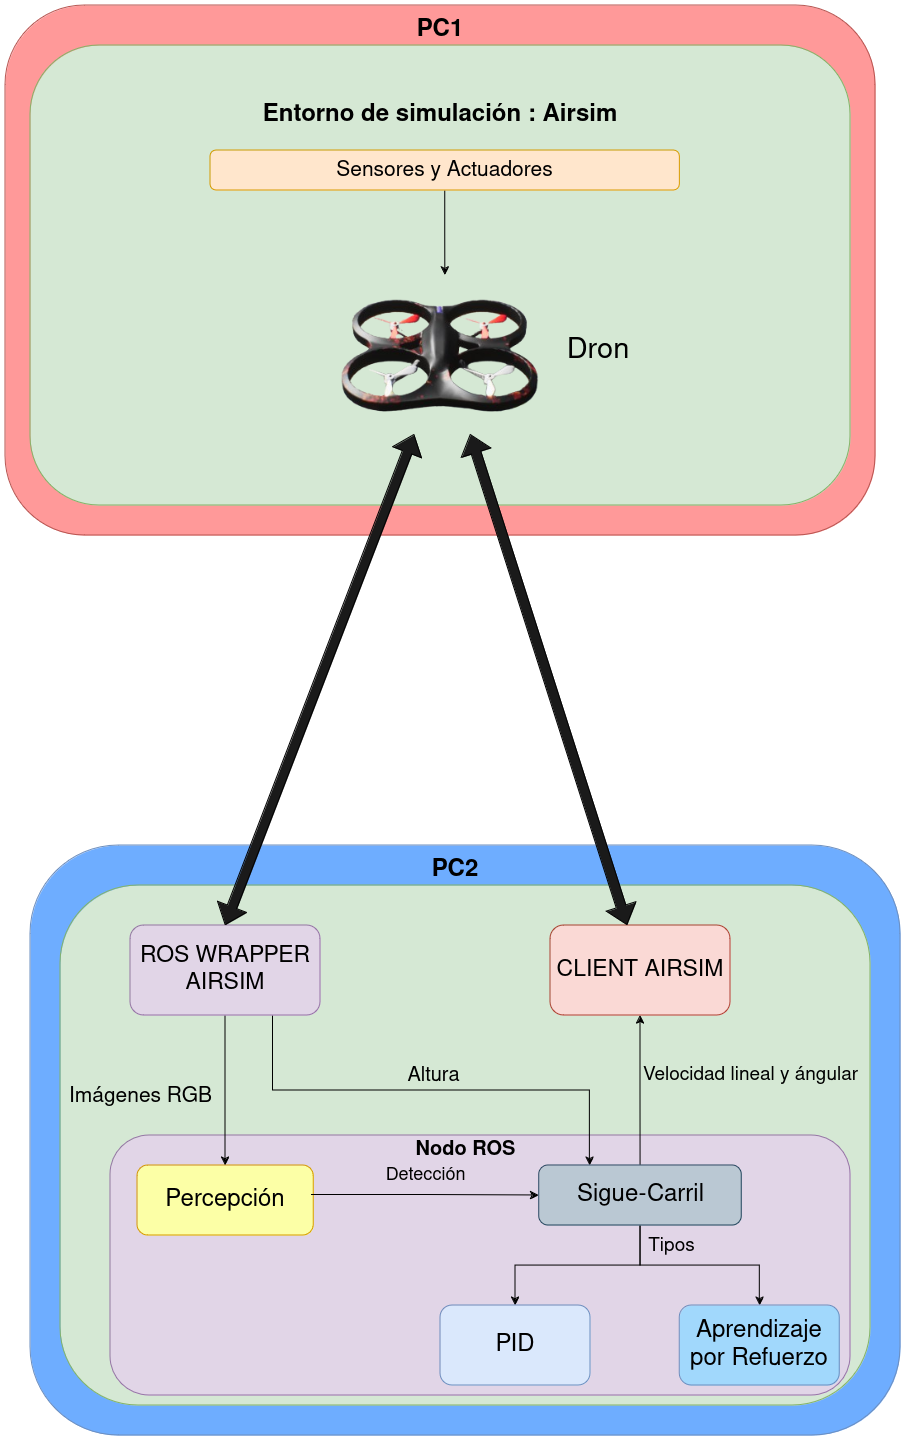
\includegraphics[scale=0.30]{figs/Diseño/Comunicaciones/digrama_arquitectura.png}
    \end{center}
    \caption{Arquitectura general del desarrollo en este TFG}
    \label{fig:infraestructura}
  \end{figure}\

\section{Configuración de Integración Distribuida en equipos separados}
En el desarrollo de este TFG, hemos tomado la decisión de tener dos enfoques:

\begin{enumerate}
  \item El entorno de simulación Airsim estará en un ordenador con un sistema operativo Windows 10, una gráfica Nvidia RTX 2070 Super con el pluggin de 
  Airsim al cargar el entorno mediante el motor UnRealEngine.
  \item Las plataformas de desarrollo como ROS, Mavros, PX4, QGC y Client Airsim API estarán un  ordenador secundario con un sistema operativo Ubuntu 20.04 con una gráfica Nvidia RTX
  2070.
\end{enumerate}

Esta propuesta fue tomada con la iniciativa de no tener encapsulado en un único componente el entorno de simulación y las plataformas de desarrollo, ya que desembocaba a tener un 
bajo rendimiento en cuanto a velocidad de procesamiento del propio entorno de simulación. La primera aproximación se llegó a construir un entorno de desarrollo con un único ordenador con una gráfica
de Nvidia RTX 2070 compuesto de un sistema operativo Linux en donde se integraba el simulador Airsim junto UnrealEngine y las plataformas de desarrollo, obteniendo una media de 60 FPS (Fotogramas por segundo)
conllevando así a tener un comportamiento lento debido a la carga de procesamiento por parte del entorno de simulación. Por causa de Airsim, esta construido sobre un motor de videojuegos, maximizando los controladores
de gráficos de NVIDIA, lo que puede afectar el rendimiento en sistemas menos optimizados. Por otro lado, si utilizamos un sistema operativo como Windows, es posible lograr un alto rendimiento debido a que Windows
tiende a asignar más recursos a las aplicaciones gráficas junto con la gráfica Nvidia, lo que puede llegar a beneficiar a Airsim. Al tener Airsim en Windows llegamos tener una media 285 FPS siendo
mucho más considerable que la primera opción con un sistema operativo Linux lo cual hace interesante tener Airsim en un entorno que tenga como sistema operativo como Windows. \newline

Por otra parte, para poder utilizar las herramientas junto con el simulador necesitaríamos Linux ya que estas herramientas de desarrollo como ROS funcionan con un sistema como Linux lo cual se necesitaría 
tener dos sistemas operativos diferentes en un mismo equipo. Como se necesitaba desarrollar una comportamiento robusto, eficiente y en tiempo real para el seguimiento de un carril con un dron se decidió
la separación en dos equipos para así conseguir el mejor rendimiento por ambas partes. \newline

El entorno de simulación Airsim se puede comunicar como hemos mencionado con PX4 y Mavros siguiendo un esquema de comunicaciones marcado por la propia página oficial de 
PX4\footnote{\url{https://docs.px4.io/main/en/simulation/}} como se muestra en la siguiete figura:

\begin{figure} [H]
  \begin{center}
    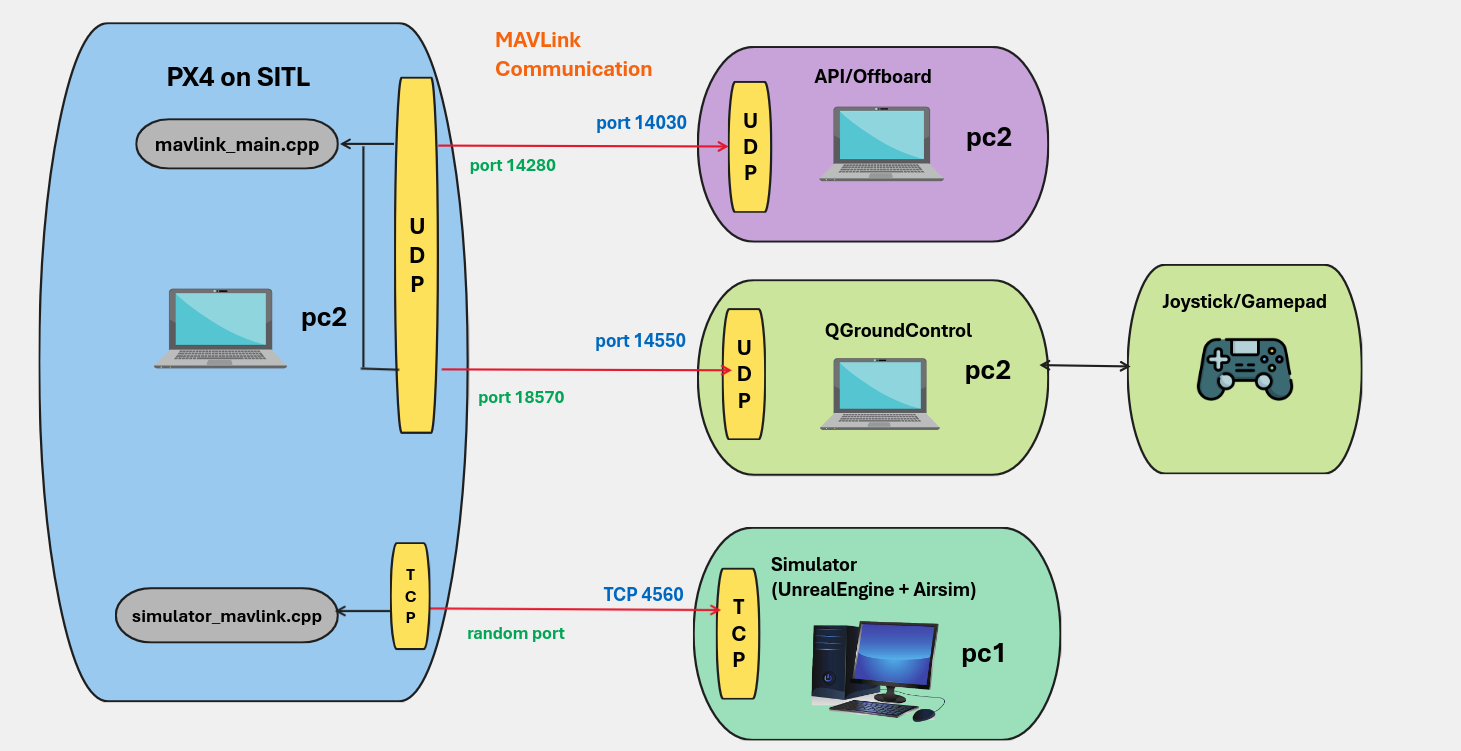
\includegraphics[scale=0.2]{figs/Diseño/Comunicaciones/diagrama_comunicaciones.png}
  \end{center}
  \caption{Diagrama de comunicaciones entre PX4, QGC y Airsim}
  \label{fig:diagramapx4}
\end{figure}\

En donde las comunicaciones internas con PX4 Autopilot se realizan mediante la ejecución del programa px4\_sitl\_default none\_iris y los puertos asignados los realiza la propia
API de Mavlink además de tener la posibilidad con PX4 de comunicarnos con QGC.

\begin{figure} [H]
  \begin{center}
    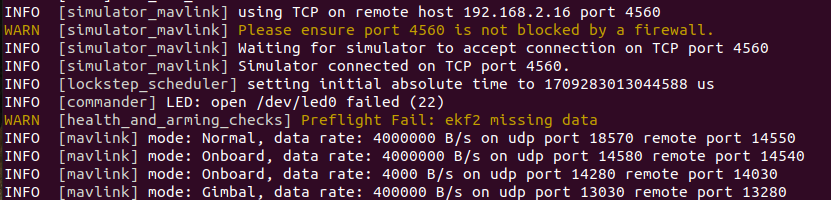
\includegraphics[scale=0.5]{figs/Diseño/Comunicaciones/puertos.png}
  \end{center}
  \caption{Salida de la terminal ejecutando PX4 SITL}
  \label{fig:SalidaTerminal}
\end{figure}\

A lo largo del desarrollo de este trabajo, nos hemos encontrado diferentes difultades respecto a la comunicación directa entre PX4 y el simulador, ya que a menudo cuando se llegaba a 
comunicar las plataformas de desarrollo entre PX4 y Airsim se producían latencias afectando a la sincronización del comportamiento autónomo que queremos desarrollar. Además de que al tener
una capa de comunicación extra con la propia herramienta PX4 Autopilot, Mavros el acceso no es totalmente directo y puede llegar a ser dificultoso. Por lo que se optó a utilizar 
Client Airsim por su comunicación directa con el simulador y se puede llegar a comunicar directamente con el simulador sin llegar a producir capas externas por su arquitectura, también
esta pensada para realizar comportamiento en tiempo real con el simulador.  \newline

En resumen, la comunicación constará de Airsim ROS Wrapper para acceder a los diferentes sensores y Client Airsim para el control del vehículo más el entorno
de simulación Airsim. El diagrama de comunicaciones que se muestra en la figura \ref{fig:diagramadeAirsim} consiste en una sencilla implementación de tener dos equipos diferentes que
constan del entorno de simulación y de las plataformas en donde iremos desarrollando los diferentes comportamientos como los algoritmos de percepción y control que serán capaces
de comunicarse entre sí en la mismo entorno de red mediante un router, cada equipo constará de dos direcciones IP diferentes. 

\begin{figure} [H]
  \begin{center}
    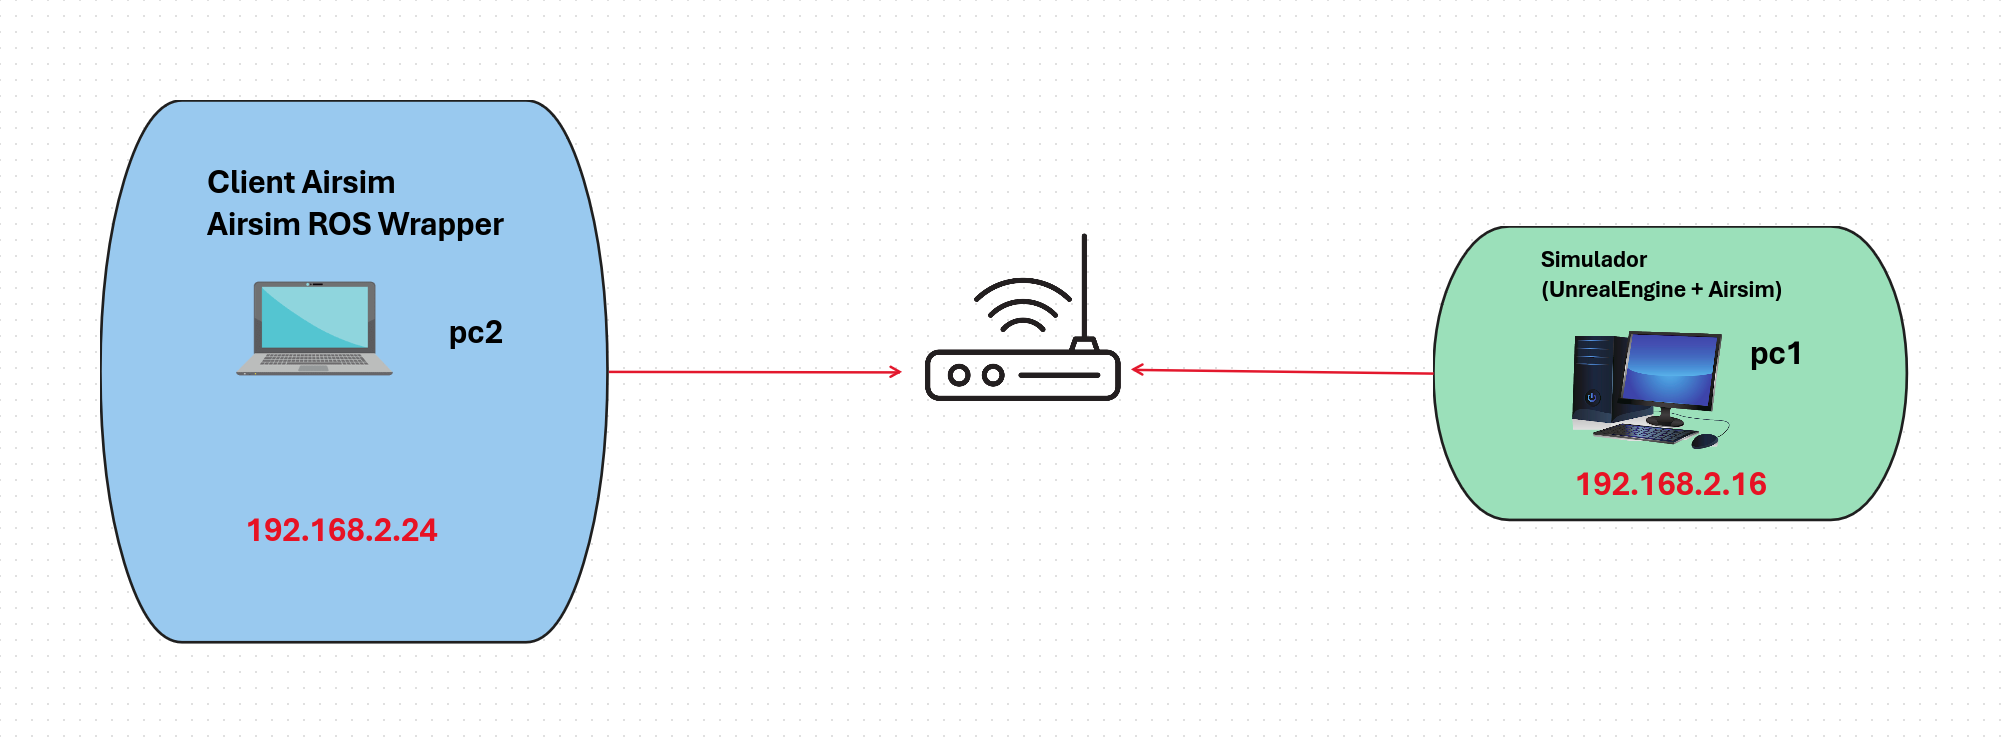
\includegraphics[scale=0.2]{figs/Diseño/Comunicaciones/Comunicaciones.png}
  \end{center}
  \caption{Diagrama de comunicaciones}
  \label{fig:diagramadeAirsim}
\end{figure}\

\section{Preparación del entorno de simulación}
\label{sec:Preparación_entorno}

Como mencionamos en la sección \ref{sec:Airsim}, utilizaremos como simulador Airsim junto con el motor UnRealEngine. Para llevar acabo la construcción del entorno, primero tendremos 
que instalar UnrealEngine. Para ello, seguiremos las instrucciones marcadas por la página oficial de Epic Games\footnote{\url{https://www.unrealengine.com/en-US/download}} y trabajaremos con la versión 4.27.2. 

Una vez se tenga UnRealEngine instalado, procederemos a configurar el entorno de simulación que necesitamos, para ello realizaremos la configuración del fichero settings.json con las diferentes
secciones. Por defecto, cuando ejecutamos por primera vez Airsim, el propio simulador nos crea este fichero dentro de una carpeta denonimada Airsim dentro de la carpeta Documentos en Windows, lo cual
es bastante cómodo ya que podemos realizar la modificación de dicho archivo a nuestras necesidades. 


\subsection{Configuración del dron y del entorno}
\label{subsec:Configuración del dron y del entorno}

En primer lugar utilizaremos el entorno de simulación Coastline de los diferentes entornos que nos ofrece Airsim para Windows. Al descargarnos dicha carpeta, contendrá el ejecutable para
poder abrir el entorno con Airsim junto con las carpetas de modelos de simulación, como las carreteras, montañas y plantas. Dentro de estas carpetas, eliminaremos dichos componentes 
de simulación que nos puede dificultar cuando desarrollemos la percepción como plantas y señales de tráfico que se ubican encima de las líneas de detección del carril ya que esto nos puede perjudicar
en un futuro en la detección con la red neuronal YOLOP.\newline
Por defecto, la primera vez que ejecutamos un entorno en Airsim, se crea el archivo settings.json en donde se almacenara por defecto en una carpeta 
llamada airsim ubicada en Documentos en Windows. \newline

\begin{figure} [H]
  \begin{center}
    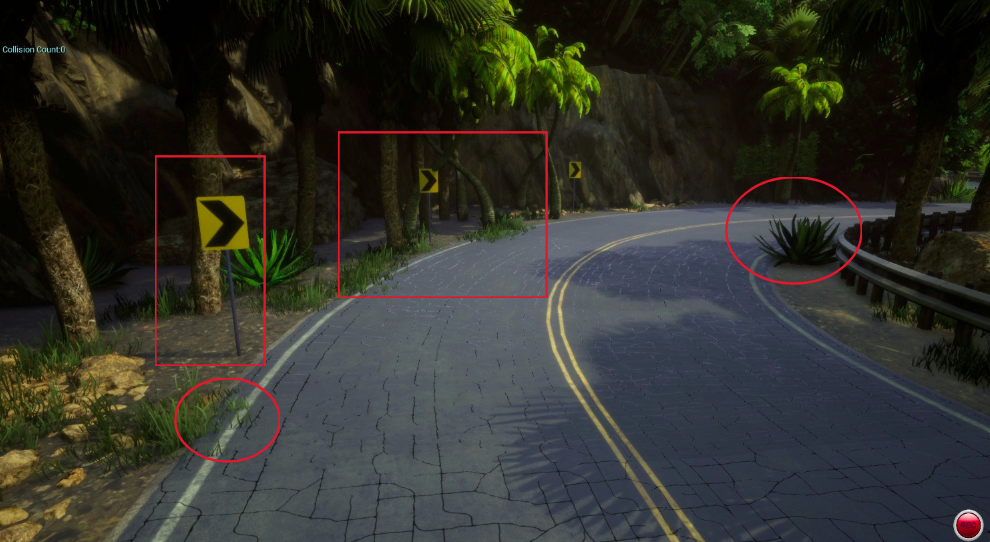
\includegraphics[scale=0.4]{figs/Diseño/coastline3.png}
  \end{center}
  \caption{Visualización del entorno original ilustrando los objetos dificultando la
  percepción de la carretera}
  \label{fig:CoastlineModificado}
\end{figure}\

Cuando tengamos el fichero settings.json creado, ya podremos equipar al vehículo con características como qué sensores utilizará, 
el tipo de vehículo, el tipo de simulación, la comunicación y más. En este TFG se definirá como sensores el lidar para saber a que altura esta volando 
el dron respecto al suelo, el gps para saber que localización tiene en el entorno y la cámara. Cada sensor debe llevar su propia configuración, como se muestra 
en el código \ref{cod:settings} se configuró cada sensor siguiendo sus propios parámetros que dicta la guía oficial de Airsim\footnote{\url{https://microsoft.github.io/AirSim/sensors/}}
. La cámara tiene una peculiaridad de que se configura siendo otro sensor a parte de la lista de sensores de Airsim, consta de varios parámetros que se tendrán que configurar como 
el tamaño de la imagen, si queremos ROS, los FPS de la imagen transmitida, la posición y más.

\begin{code}[H]
  \begin{lstlisting}[language=json,basicstyle=\tiny]
    {
      "SettingsVersion":1.2,
      "SimMode":"Multirotor",
      "ClockType":"SteppableClock",
      "Vehicles":{
         "Drone":{
            "VehicleType":"SimpleFlight",
            "ControlIp":"remote",
            "LocalHostIp":"192.168.2.16",
            "Sensors":{
               "LidarCustom":{
                  "SensorType":6,
                  "Enabled":true,
                  "Range":10,
                  "NumberOfChannels":16,
                  "RotationsPerSecond":10,
                  "PointsPerSecond":10000,
                  "X":0,
                  "Y":0,
                  "Z":-1,
                  "DrawDebugPoints":false,
                  "DataFrame":"SensorLocalFrame"
               },
               "Gps":{
                  "SensorType":3,
                  "Enabled":true,
                  "EphTimeConstant":0.9,
                  "EpvTimeConstant":0.9,
                  "EphInitial":25,
                  "EpvInitial":25,
                  "EphFinal":0.1,
                  "EpvFinal":0.1,
                  "EphMin3d":3,
                  "EphMin2d":4,
                  "UpdateLatency":0.2,
                  "UpdateFrequency":50,
                  "StartupDelay":1
               }
            },
            "Cameras":{
               "front_center_custom":{
                  "CaptureSettings":[
                     {
                        "PublishToRos":1,
                        "ImageType":0,
                        "Width":620,
                        "Height":620,
                        "FOV_Degrees":90,
                        "ImageRate_FPS":30,
                        "TargetGamma":1.5,
                        "AutoExposure":true,
                        "MotionBlur":false,
                        "PostProcess":true
                     }
                  ],
                 
                  "X":0.50,
                  "Y":0,
                  "Z":0.10,
                  "Pitch":0,
                  "Roll":0,
                  "Yaw": 0
               }
            },
         "X": 22.474933624267578,
         "Y": -25.63629913330078,
         "Z":  0,
         "Pitch": 0,
         "Roll": 0,
         "Yaw":  30
         }
      }
   }

  \end{lstlisting}
  \caption[Configuración del vehículo mediante el fichero settings.json]{Configuración del vehículo mediante el fichero settings.json}
  \label{cod:settings}
  \end{code}  

Si no se define la posición inicial del dron como aparece en la última parte del fichero settings.json, por defecto el propio simulador te establece el vehículo en el punto que decida Airsim. 



  \subsection{Instalación de las herramientas de desarrollo}
  \label{subsec:Instalación de las herramientas de desarrollo}
  La instalación de las herramientas de desarrollo se realizarán en el segundo ordenador con el sistema operativo Linux.
  \begin{enumerate}
    \item \textbf{ROS}: Como se menciona en la documentación oficial de ROS \cite{Dis_ROS}, ROS consta de diferentes conjuntos de paquetes versionados que permiten a los desarrolladores
    trabajar con un código relativamente estable hasta que estén preparados y puedan publicar versiones robustas y eficientes. En nuestro caso, utilizaremos la distribución Noetic\footnote{\url{http://wiki.ros.org/noetic}}
    debido a que esta distribución se encuentra siendo una de las más estables para poder trabajar junto con Airsim\footnote{\url{https://microsoft.github.io/AirSim/airsim_ros_pkgs/}}.

    Para su instalación nos guiaremos en la guía oficial de ROS noetic\footnote{\url{https://wiki.ros.org/noetic/Installation/Ubuntu}}

    \begin{figure} [H]
      \begin{center}
        
\includegraphics[scale=0.3]{figs/Plataformas_Desarollo/ros-noetic.png}
      \end{center}
      \caption{Logotipo de ROS noetic}
      \label{fig:ROS noetic}
    \end{figure}\
    \item \textbf{Airsim ROS Wrapper}: Descargaremos del repositorio de Airsim a través de su página de github\footnote{\url{https://github.com/microsoft/AirSim}}.
    Cuando tengamos dicho repositorio descargado, lo que realizaremos será la compilación y configuración de Airsim mediante los scripts build y setup como se pauta en la guía oficial. \newline
    \begin{code}[H]
      \begin{lstlisting}
        git clone https://github.com/microsoft/AirSim.git
      \end{lstlisting}
      \caption[gitclone]{Comando para poder clonar el repositorio de Airsim}
      \label{cod:gitclone}
    \end{code}
  
    Ahora para poder utilizar el Airsim ROS Wrapper que nos proporciona ROS, tendremos que irnos a la carpeta dentro del repositorio de Airsim clonado previamente y buscar la carpeta de ros y construir el paquete 
    mediante el comando \texttt{catkin\_make}. Cuando tengamos realizado dicho paso tendremos que activar el wrapper en el fichero .bashrc de Linux mediante la siguiente linea: \newline

    \begin{code}  [H]
      \begin{lstlisting}
        source /home/$USER/Airsim/ros/devel/setup.bashrc
      \end{lstlisting}
      \caption[bash]{Comando para activar el entorno de trabajo en el fichero bashrc}
      \label{cod:bashrc}
    \end{code} 


     siendo \$USER la variable de entorno que contiene el nombre del usuario que actualmente tiene iniciada sesión en el equipo.

     A partir de activar el entorno de trabajo para ros, utilizaremos el nodo AirSim ROS Wrapper Node \ref{sec:wrapper} junto con un launcher airsim\_node.launch proporcionando
     la dirección IP en donde se encuentra Airsim.\newline

     \begin{code}  [H]
      \begin{lstlisting}
        roslaunch airsim_ros_pkgs airsim_node.launch output:=screen host:=192.168.2.16
      \end{lstlisting}
      \caption[comando]{Lanzamiento del nodo AirSim ROS Wrapper Node especificando la dirección IP del simulador}
      \label{cod:roslaunch}
    \end{code} 

  \end{enumerate}

\section{Percepción}
\label{sec:Percepción}
Para el desarrollo de la percepción una primera aproximación fue utilizar
procedimientos de visión clásica, es decir, procesar la imagen y mediante métodos de la librería OpenCV
poder detectar las diferentes líneas que pueden haber en la carretera. El problema que nos podemos con esta primera proximación que al tener un 
entorno fotorrealista, estos métodos se quedan bastante pobres desembocando una percepción muy poco robusta e ineficiente. Por lo que se optó la utilización
de la red neuronal YOLOP y algoritmos de aprendizaje automático poder construir la percepción. \newline

Para obtener la imagen del entorno, nos subscribiremos al topic /airsim\_node/Drone/front\_center\_custom/Scene que ofrece el nodo AirSim ROS Wrapper Node
 y mediante un método de ROS denominado CvBridge\footnote{\url{http://wiki.ros.org/cv_bridge}} podremos convertir dicha imagen en formato OpenCV y trabajar con ella a traves de OpenCv.\newline

\subsection{Inferencia de YOLOP}
\label{sec:Inferencia de YOLOP}

Para realizar la deteción de las líneas en la carretera nos vamos ayudar de la red neuronal YOLOP\ref{sec:YOLOP}. En primer lugar, 
como anteriormente hemos comentado, el archivo End-to-end.pth es un archivo de pesos construido en Pytorch, si queremos cargar
dichos pesos con el modelo podemos hacerlo de dos maneras: Podemos realizarlo mediante la CPU o la GPU. 
Para ello, si queremos cargar el modelo de YOLOP con los pesos preentrenados End-to-end.pth se realiza la carga del modelo de la red a través de su repositorio de github\footnote{\url{https://github.com/hustvl/YOLOP}}
especificando el modelo de la red neuronal y la opción 'pretrained' colocada con valor True, especificando que los pesos del modelo de la red se cargan del archivo End-to-end.pth en formato pytorch.\newline
\begin{code}[h]
  \begin{lstlisting}[language=Python]
  import torch
  
  model = torch.hub.load('hustvl/yolop', 'yolop', pretrained=True)

  \end{lstlisting}
  \caption[Cargar modelo YOLOP con pesos preentrenados End-to-end.pth]{Cargar modelo YOLOP con pesos preentrenados End-to-end.pth}
  \label{cod:cargar_modelo}
  \end{code}  

Una vez tengamos el modelo cargado del repositorio como se ilustra en el código \ref{cod:cargar_modelo}, podemos escoger si queremos hacer la inferencia en la CPU o GPU, tendremos que especificar como 
lo queremos hacer. En nuestro, escogemos la opción de GPU para realizar la inferencia y se le asigna al modelo que realizaremos la inferencia por GPU 
como se muestra en el código \ref{cod:codeloadYOLOP}.\newline

  
  \begin{code}[h]
    \begin{lstlisting}[language=Python]
   
    device = torch.device("cuda" if torch.cuda.is_available() else "cpu")
    model = model.to(device)
  
    \end{lstlisting}
    \caption[Cargar modelo YOLOP escogiendo como disposivo la GPU]{Cargar modelo YOLOP escogiendo como disposivo la GPU}
    \label{cod:codeloadYOLOP}
    \end{code}  

    Por último, nos quedaria convertir la imagen en un tensor antes de realizar la inferencia. Para poder realizarlo, se utiliza la función transforms.toTensor\footnote{\url{https://pytorch.org/vision/main/generated/torchvision.transforms.ToTensor.html}} 
    y después añadiremos una dimensión más con unsqueeze(0) como se muestra en el código \ref{cod:Inferencia}, esto se debe 
    a que el modelo de YOLOP espera una entrada específica llamada batch\_size. Batch\_size es el número de imágenes que se procesarán juntas
    (generalmente 1 para inferencia) por lo que el tensor tendrá esta forma: (batch\_size, channels, height, width)\newline

    \begin{code}[h]
      \begin{lstlisting}[language=Python]
     
        from torchvision import transforms

        transform = transforms.ToTensor() 
                    
      imagen_tensor = transform(cv_image).to(device).unsqueeze(0)
      _, da_seg_out, ll_seg_out = self.model(imagen_tensor)
    
      \end{lstlisting}
      \caption[Inferencia del modelo]{Inferencia del modelo en Pytorch}
      \label{cod:Inferencia}
      \end{code}  

    Como resultado de la inferencia se obtiene un tensor de salida que corresponde la probabilidad de detección de la segmentación
    de la calzada y la detección de las líneas de la calzada. Dicho tensor se debe de convertir en una imagen para poder visualizar
    dicho resultado como una imagen. 
    Por ello, se convierte el tensor en un array numpy y se realiza una transformacion para cambiar las dimensiones de (H,W,C) 
    a (C,H,W) esto se realiza ya que en Opencv representa imágenes en formato numpy array y se transpone las dimensiones porque las
    imágenes de Opencv tiene la forma de (H, W, C)\footnote{\url{https://lindevs.com/convert-pytorch-tensor-to-opencv-image-using-python}}. 

    Después de este proceso,obtenemos un array de numpy que se normaliza con valores de 0-1. La normalización 
    ayuda a igualar la escala de los pixeles de la imagen. Finalmente se muestra el resultado de la inferencia de la red 
    en una imagen como se ilustra en el codigo \ref{cod:Resultadoinferencia}. Al normalizar los valores de 0-1, los pixeles con un valor 1 se muestran en la imagen final, asignándoles un color
    para visualizar el resultado de la segmentación de la calzada y de la detección de las líneas de la calzada. \newline
    \newpage
    \begin{code}[h]
      \begin{lstlisting}[language=Python]
        import cv2
        import numpy as np
        for image in (da_seg_out,ll_seg_out):

          image_np = image.detach().cpu().numpy()
          image_array = np.transpose(image_np, (2, 3, 1, 0))

        
          image_norm = cv2.normalize(image_array[:,:,1,:], None, 0,1, cv2.NORM_MINMAX, cv2.CV_8U)

          images.append(image_norm)

    
        cv_image[images[0] == 1] = [0, 255, 0]
        cv_image[images[1] == 1] = [0, 0, 255]

        cv2.imshow('Image', cv_image)
        cv2.waitKey(1)

    
      \end{lstlisting}
      \caption[Resultado de la inferencia del modelo YOLOP]{Inferencia de YOLOP mediante los pesos End-to-end.pth}
      \label{cod:Resultadoinferencia}
      \end{code}  

      Para poder utilizar los pesos preentrenados de Onnx, tendremos que realizar la configuración de los drivers de CUDA con la versión disponible para Onnx Runtime, 
      dichas versiones tienen que ser compatible entre sí. Para ello nos vamos a guiar mediante la tabla requisitos de la página oficial de Onnx Runtime\footnote{\url{https://onnxruntime.ai/docs/execution-providers/CUDA-ExecutionProvider.html}}. \newline

      Cuando tengamos todo preparado y configurado ya podremos realizar los pasos de la inferencia con los pesos preentrenados de Onnx. En primer lugar, se carga el modelo
      
      \begin{code}[h]
        \begin{lstlisting}[language=Python]
          import onnxruntime as ort

          ROUTE_MODEL = "/home/bb6/YOLOP/weights/yolop-320-320.onnx"
          ort_session = ort.InferenceSession(ROUTE_MODEL,providers=['CUDAExecutionProvider'])
      
        \end{lstlisting}
        \caption[Cargar modelo]{Cargar modelo por ejemplo YOLOP-320-320.onnx}
        \label{yolop320}
        \end{code}  

        Como se observa en el código \ref{yolop320}, a la hora de cargar el modelo escogemos como provider CUDAExecutionProvider. Cuando trabajamos con ONNX Runtime, 
        podemos especificar qué proveedores de ejecución utilizar para ejecutar el modelo ONNX que escojamos, cada proveedor contiene un conjunto de núcleos optimizados para un objetivo específico (por ejemplo, CPU, GPU, IoT) y 
        se especifican como una lista en el orden de prioridad. En nuestro caso escogemos CUDA para ejecutar mediante la GPU. 
        \newline
        A continuación se procesan las imágenes de entrada que le vamos a dar al modelo, al escoger el modelo de yolop-320-320.onnx, las imágenes deben tener una dimensión de 320x320, para ello
        se utiliza un método implementado por ellos que se puede encontrar en la siguiente página\footnote{\url{https://debuggercafe.com/yolop-onnx-inference-on-cpu}}, en el cuál se redimensiona la imagen como se pide para el modelo. 
        Una vez que tengamos la imagen preparada, se da pie a la inferencia del modelo de yolop-320-320.onnx como se ilustra en el código \ref{cod:Inferencia_onnx}. \newline
      
        \begin{code}[h]
          \begin{lstlisting}[language=Python]
            _, da_seg_out, ll_seg_out = self.ort_session.run(
              ['det_out', 'drive_area_seg', 'lane_line_seg'],
              input_feed={"images": img}
          )
        
          \end{lstlisting}
          \caption[Inferencia del modelo yolop-320-320.onnx]{Inferencia del modelo yolop-320-320.onnx}
          \label{cod:Inferencia_onnx}
          \end{code}  

        La inferencia del resto de modelos de Onnx se realizan de la misma forma pero teniendo en cuenta que se tendrá que cambiar las dimensiones de las imágenes de entrada y la ruta
        en donde se almacena dicho modelo. 


\subsubsection{Resultados de YOLOP }
\label{sec:resultados}
En esta sección se constrastan los resultados de los diferentes pesos preentrenados que ofrece la red neuronal YOLOP. Como podemos observar en la figura \ref{fig:resultados_pesos_preentrenados} 
mostramos la media en realizar la inferencia de YOLOP utilizando los pesos preentrenados End-to-end.pth, yolop-320-320.onnx,yolop-640-640.onnx e yolop-1280-1280.onnx en segundos.

\begin{figure} [H]
  \begin{center}
    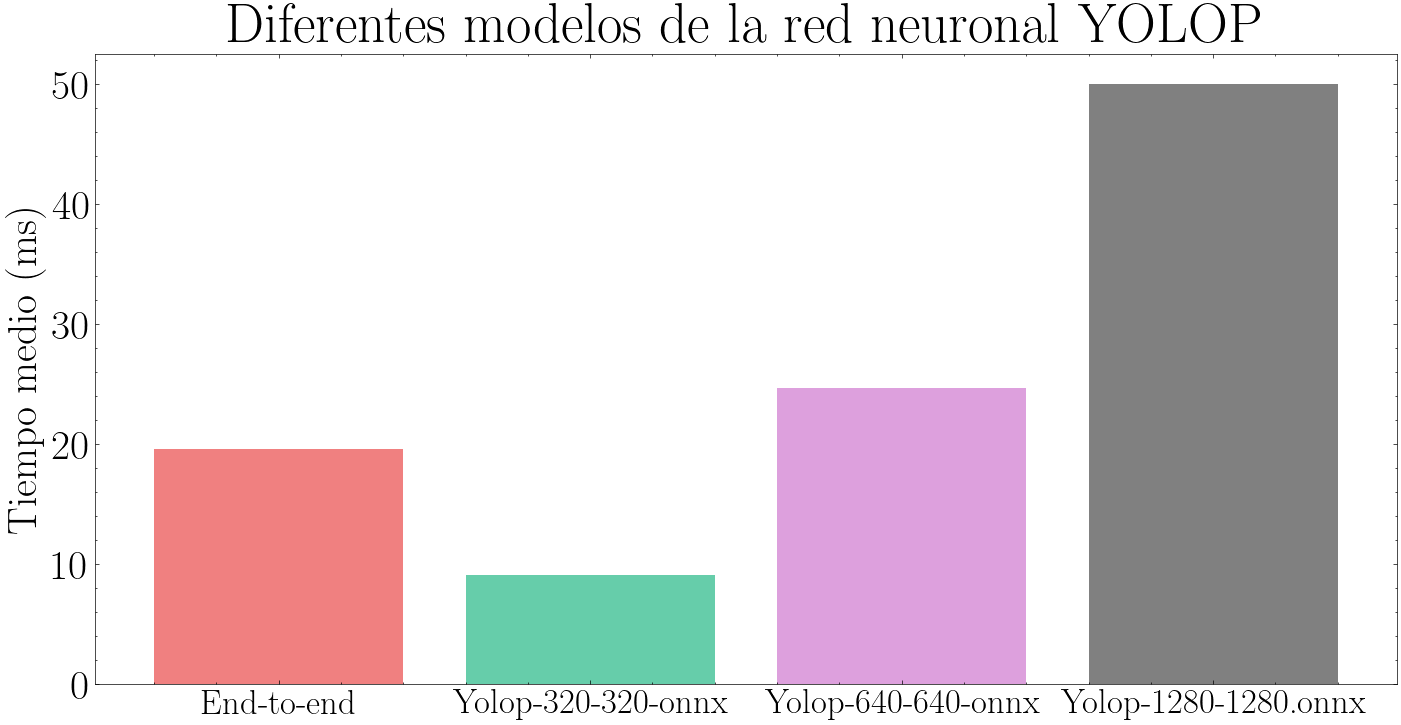
\includegraphics[scale=0.4]{figs/Diseño/YOLOP/comparativa.png}
  \end{center}
  \caption{Resultados de los diferentes pesos que ofrece el modelo YOLOP}
  \label{fig:resultados_pesos_preentrenados}
\end{figure}\

Los pesos preentrenados que tiene una inferencia menor al resto se trata de yolop-320-320.onnx, tiene un tiempo de inferencia alrededor de 0.010 segundos, esto
significa que el modelo YOLOP con estos pesos tiene aproximadamente un rate de 100 FPS. Si comparamos este resultado con los restantes pesos, es el ganador en cuanto 
en tiempo de inferencia, rate y mejores resultados. 
Onnx está diseñado para ser más eficiente en términos de memoria y velocidad de inferencia en cuanto Pytorch, lo que puede mejorar la velocidad y la precisión
del modelo, una menor resolución en cuanto al tamaño de las imágenes reduciendo la cantidad de información al procesarlas. Aun así, depende de varios factores y según las necesidades, nosotros
buscamos un equilibrio entre velocidad de inferencia y mejores resultados en cuanto a la detección de las líneas de la calzada. 
Por ello nos decantamos por escoger el modelo yolop320-320.onnx ya que obtiene mejores resultados para poder realizar la detección de las líneas del carril que 
queremos segir como se aprecia en la figura \ref{f:resultadosYOLOP}.\newline

\begin{figure}[H]
  \begin{center}
    \subfigure[yolop-320-320.onnx]{
     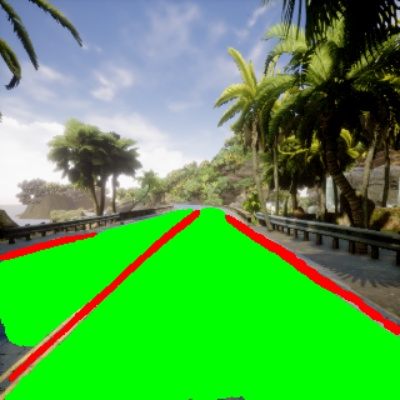
\includegraphics[scale=0.4]{figs/Plataformas_Desarollo/resultados-yolop/sitio1/ONNX-320-320.jpg}
     \label{f:Yolop-320-320.onnx}}
    \subfigure[yolop-640-640.onnx]{
      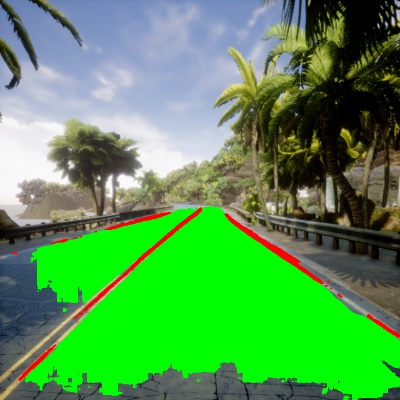
\includegraphics[scale=0.4]{figs/Plataformas_Desarollo/resultados-yolop/sitio1/ONNX-640-640.jpg}
      \label{yolop-640-640.onnx}}
    \subfigure[yolop-1280-1280.onnx]{
      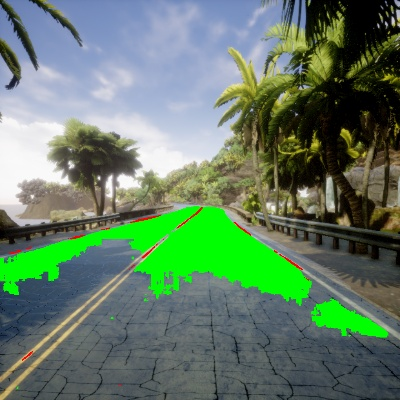
\includegraphics[scale=0.4]{figs/Plataformas_Desarollo/resultados-yolop/sitio1/ONNX-1280-1280.jpg}
      \label{f:yolop-1280-1280.onnx}}
    \subfigure[end-to-end.pth]{
      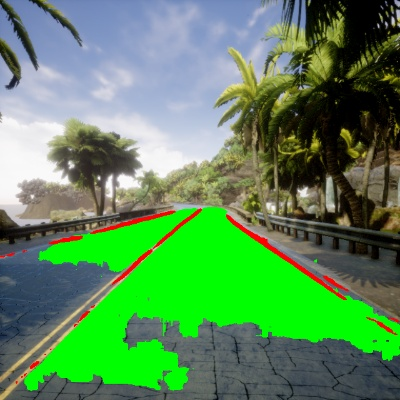
\includegraphics[scale=0.4]{figs/Plataformas_Desarollo/resultados-yolop/sitio1/Pytorch.jpg}
      \label{f:End-to-end.pth}}
  \caption{Diferentes resultados utilizando la red neuronal YOLOP en el entorno de simulación}
  \label{f:resultadosYOLOP}
  \end{center}
 \end{figure}

Finalizado este proceso, se procede a seleccionar las líneas detectadas que nos interesan mediante un algoritmo de aprendizaje no supervisado denonimado clustering.

\subsection{DBSCAN}
\label{sec:DBSCAN}

Para saber con qué líneas detectadas por la red nos quedaremos, utilizamos un algoritmo de aprendizaje no supervisado llamado clustering, en particular
DBSCAN(Density-Based Spatial Clustering of Applications with Noise)\cite{ski_dbs}.\newline

Dicho algoritmo contiene varios parámetros que son importantes conocerlos y configurarlos: 
\begin{enumerate}
  \item \textbf{Eps}: Consiste en la distancia máxima que puede existir entre dos muestras para que una se considere vecina de la otra. Dicha distancia no se trata de un límite 
  máximo entre las distancias que puede haber dentro de un cluster.
  \item \textbf{Min\_samples}: Es el número mínimo de muestras dentro de un vecindario para que un punto se considere como un punto central incluyendo al propio punto.
  \item \textbf{Metric}: La métrica utilizada para calcular la distancia entre los conjuntos de clústeres (por defecto es la distancia euclidiana). 
\end{enumerate}
Los valores de los parámetros de la distancia máxima y el número mínimo de muestras se deben elegir cuidadosamente, es decir, si colocamos una distancia 
máxima alta puede provocar que los clústeres que queramos que pertenezcan a un distinto grupo pertenezcan al mismo grupo. 
Si min\_samples se establece en un valor alto, DBSCAN encontrará clústeres más densos y 
si se establece en un valor bajo, los clústeres encontrados serán más dispersos. \newline
Para entender como funciona el algoritmo, en la figura \ref{fig:Ejemplo_DBSCAN} recogida por este artículo\cite{DBSCAN} se ilustra 
un ejemplo teniendo un número de muestras ubicadas aproximadamente cercanas unas de otras. Aplicamos el algoritmo de DBSCAN 
teniendo como valor el número mínimo de muestras 3, eso significa que para que se considere una muestra a un grupo de cluster tendrá que tener una densidad de 3. El algoritmo itera por
las muestras y compara el valor de la distancia máxima y el número mínimo de muestras. 
Si ningún de estos dos parámetros no se cumpliese ya que puede darse que una muestra se encuentra lejana del grupo de muestras será etiquetado como ruido, esto quiere decir
que no pertenecerá a ningún grupo de clústeres. El resultado del algoritmo ha catalogado dos grupos de clústeres y 3 muestras. \newline

\begin{figure} [H]
  \begin{center}
    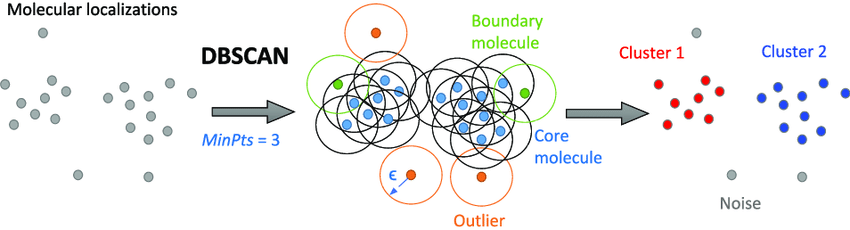
\includegraphics[scale=0.5]{figs/Diseño/DBSCAN/DBSCAN-Illustration.png}
  \end{center}
  \caption{Ejemplo ilustrativo de como funciona el algoritmo de DBSCAN \cite{DBSCAN}}
  \label{fig:Ejemplo_DBSCAN}
\end{figure}\

Por lo que para encontrar los valores de estos dos parámetros durante el desarrollo del TFG fue experimental y quedándonos con el mejor resultado. La distancia máxima tiene un valor de 10 
y el número mínimo de muestras son de 5 muestras. Lo que significa que la distancia máxima que tienen los puntos para pertenecer al mismo grupo de clústeres es de 10 de distancia en pixeles
con un mínimo de muestras pertenecientes de 5 muestras como se muestra en el código \ref{cod:DBSCAN}. Para poder aplicar este algoritmo a partir del resultado de la imagen de la red neuronal se convierte la imagen resultante
de la red neuronal en un array bidimensional de coordenadas x e y de puntos con la ayuda de la función de numpy column\_stack\footnote{\url{https://numpy.org/doc/stable/reference/generated/numpy.column_stack.html}}, 
transformando un array simple de una dimensión a un array de dos dimensiones. Una vez se realice lo anterior, se obtiene un array bidimensional listo para el algoritmo DBSCAN .\newline


\begin{code}[h]
  \begin{lstlisting}[language=Python]
    def clustering(self,cv_image):

    #--Convert image in points
    points_lane = np.column_stack(np.where(cv_image > 0))
    dbscan = DBSCAN(eps=10, min_samples=5,metric="euclidean")
    

    if points_lane.size > 0:
        dbscan.fit(points_lane)
        labels = dbscan.labels_

        # Ignore noise if present
        clusters = set(labels)
        if -1 in clusters:
            clusters.remove(-1)
      
      
            
        for cluster in clusters:
            points_cluster = points_lane[labels==cluster,:]
            centroid = points_cluster.mean(axis=0).astype(int)
            color = self.colors[cluster % len(self.colors)]
            cv_image[points_cluster[:,0], points_cluster[:,1]] = color

        return cv_image
  
  \end{lstlisting}
  \caption[Algoritmo de custering utilizando DBSCAN]{Algoritmo de clustering utilizando DBSCAN}
  \label{cod:DBSCAN}
  \end{code}  
  

El resultado de DBSCAN es una lista con etiquetas de 0 a n, siendo 0 el primer grupo de clusters detectado y 
n el último grupo de clusters detectado. De las listas de etiquetas se eliminan los clusters que hallan sido etiquetados como ruido (-1). Para obtener el resultado solamente basta con iterar en dicha lista y mostrar los puntos correspondientes de cada etiqueta en la imagen de salida.
Visualmente se puede apreciar en la figura \ref{f:Rresultadosdbscan} los diferentes resultados que tiene este algoritmo en localizaciones distintas. 

\begin{figure}[H]
  \begin{center}
    \subfigure[DBSCAN zona 1]{
     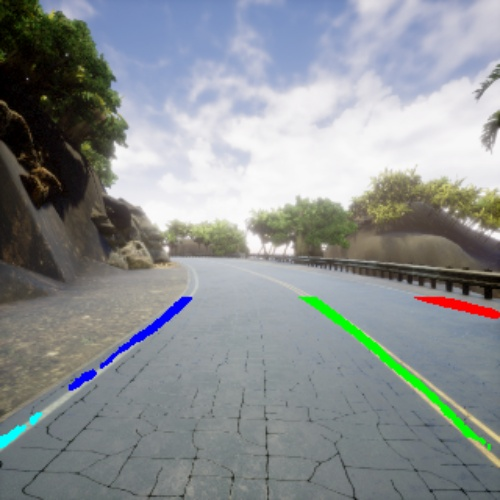
\includegraphics[scale=0.4]{figs/Diseño/DBSCAN/dbscan1.jpg}
     \label{f:dbcan1}}
    \subfigure[DBSCAN zona 2]{
      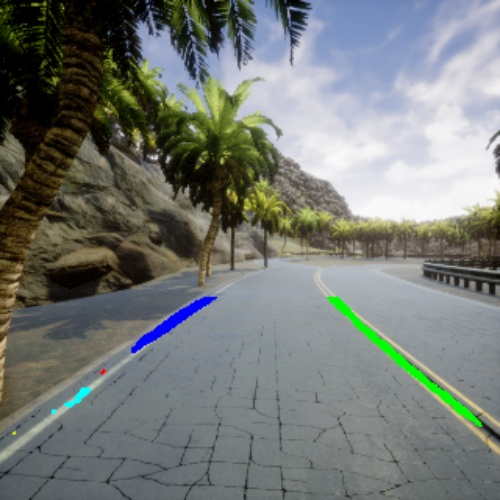
\includegraphics[scale=0.4]{figs/Diseño/DBSCAN/dbscan2.jpg}
      \label{f:dbcan2}}
    \subfigure[DBSCAN zona 3]{
      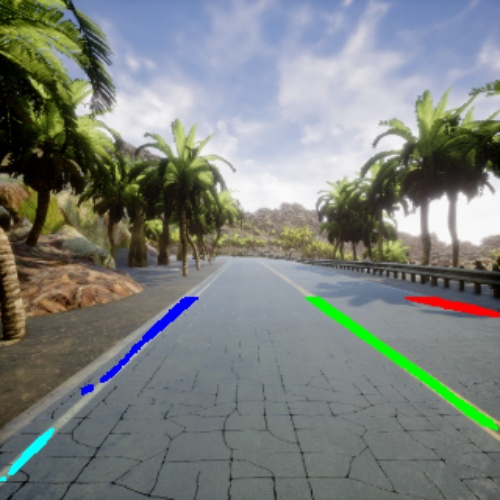
\includegraphics[scale=0.4]{figs/Diseño/DBSCAN/dbscan3.jpg}
      \label{f:dbcan3}}
  \caption{Diferentes resultados utilizando el algoritmo de DBSCAN con valor de eps de 10 y valor de min\_samples de 5}
  \label{f:Rresultadosdbscan}
  \end{center}
 \end{figure}



\subsection{Clasificación de clústeres}
\label{clasificación:cluster}
Una vez realizado el algoritmo de DBSCAN necesitamos quedarnos con el grupo de clústeres que pertenezcan al carril que queremos seguir. Para conseguirlo, se calcula los centroides de cada
grupo de clústeres detectado y los clasificaremos en función de sí se encuentran en la derecha o izquierda respecto al centro de la imagen. La imagen tiene unas dimensiones de 320x320 píxeles, 
siendo su centro (160,160) pixeles, x = 160 e y = 160. Nos fijaremos solamente en los valores de x de los centroides para poder clasificarlos en función del centro de la 
imagen, a partir de ello serán divididos en dos grupos distinguidos: derecha e izquierda de la imagen como se muestra en el código \ref{cod:Clasificación de clústeres}. \newline

\begin{code}[h]
  \begin{lstlisting}[language=Python]
    # Check if the centroid is within the desired lane

    WIDTH = cv_image.shape[1]
    if centroid[1] < WIDTH/2:  # left lane
        left_clusters.append((points_cluster,centroid))
       
    elif centroid[1] >= WIDTH/2:  # right lane
        right_clusters.append((points_cluster, centroid))
       
  
  \end{lstlisting}
  \caption[Clasificación de clústeres según las dimensiones de la imagen ]{Clasificación de clústeres respecto a las dimensiones de la imagen}
  \label{cod:Clasificación de clústeres}
  \end{code}  


Cuando sean clasificados los grupos de los clústeres, necesitamos quedarnos con qué subgrupo de cada grupo de clústeres (izquierda e derecha) nos queremos quedar respecto al carril. Esogemos dichos grupos mediante una función máximizada 
respecto a un punto central P predefinido con valor (220,160) siendo 220 el valor de las y e 160 el valor de las x, dichos valores son calculados respecto 
a las dimensiones de la imagen 320x320 píxeles. Es importante mencionar que cuando trabajamos con puntos en numpy las coordenadas estan opuestas, es decir, en vez de tener el formato (x,y) como estamos acostumbrados a trabajar tienen el formato(y,x). 
A parte de escoger lo sugrupos respecto a un punto central P también se realiza en función de la densidad de puntos de dicho grupo de clústeres de la derecha u izquierda detectados, 
con esto conseguimos que no solamente se escoja en función de la cercania si no que también lo haremos según la cantidad de puntos. El proceso se ilustra 
en el código \ref{cod:funcion_maximizada}.\newline

\begin{code}[h]
  \begin{lstlisting}[language=Python]
    def score_cluster(self,cluster, center):
      points_cluster, centroid = cluster
    
      proximity = np.linalg.norm(centroid - center)
      density = len(points_cluster)
      return density / proximity

  \end{lstlisting}
  \caption[Función maximizada para escoger el grupo de cluster más cercano y denso respecto al punto P]{Función maximizada para escoger el grupo de cluster más cercano y denso respecto al punto P}
  \label{cod:funcion_maximizada}
  \end{code}  

  En la figura \ref{fig:DBSCAN_imagen} se muestra todo el proceso desde el uso del algoritmo de DBSCAN hasta la clasificación de clústeres respecto al carril 
  representados en color verde y rojo. Después de tener la clasificación de los grupos de clústeres se procede a realizar dos regresiones cuadráticas para construir las líneas del carril que queremos seguir.

\begin{figure} [H]
  \begin{center}
    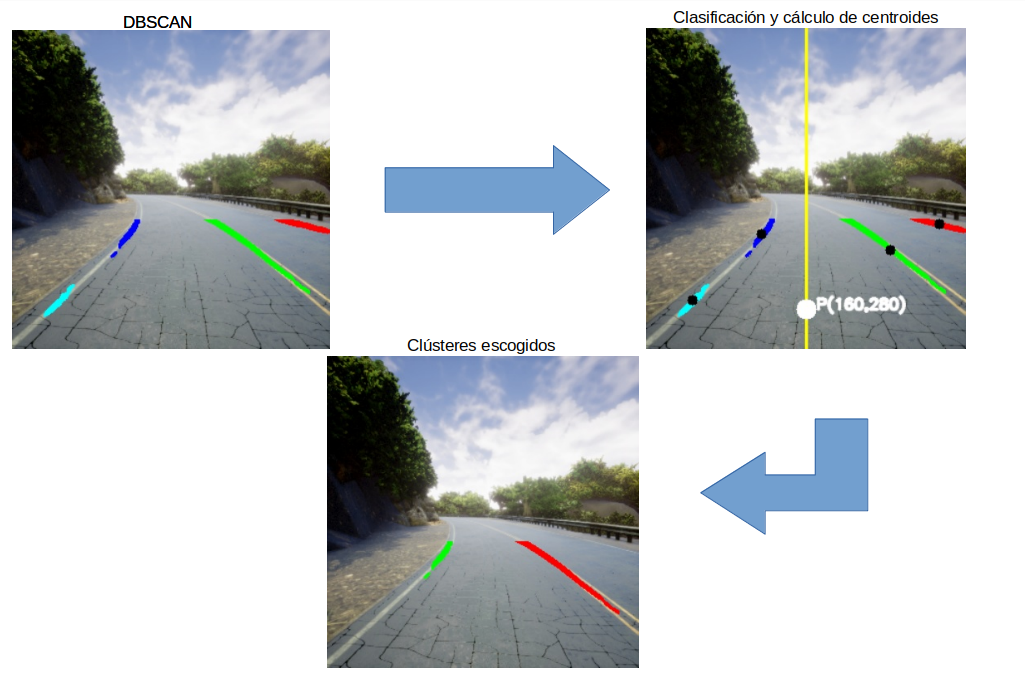
\includegraphics[scale=0.5]{figs/Diseño/DBSCAN/resultado.png}
  \end{center}
  \caption{Ilustración del proceso de clasificación de líneas detectadas respecto al carril que queremos seguir}
  \label{fig:DBSCAN_imagen}
\end{figure}\

\subsection{Regresión cuadrática}
\label{sec:Regresión cuadrática}
Como anteriormente hemos mencionado, cuando se clasifique los clústeres correctamente daremos pie a la construcción de dos regresiones cuadráticas. \newline 

La regresión es un método de aprendizaje supervisado el cual consiste en aproximar un número N de puntos a una recta, curva, etc, en nuestro caso hemos escogido realizar una regresión cuadrática ya que el recorrido
que vamos a realizar las líneas detectadas por la red neuronal no son totalmente rectas si no que se tratan de líneas curvilíneas por lo que la regresión cuadrática en este papel puede 
funcionar perfectamente. 
Para la construcción de las regresiones cuadráticas se utiliza las funciones de la librería numpy denominada Polyfit\footnote{\url{https://numpy.org/doc/stable/reference/generated/numpy.polyfit.html}}
y Polyval\footnote{\url{ https://numpy.org/doc/stable/reference/generated/numpy.polyval.html}}. 
Polyfit es una función que calcula los coeficientes del polinomio que mejor se ajusta a los datos utilizando el método de los mínimos 
cuadrados para la ecuación cuadrática,obteniendo tres coeficientes, denominados a,b y c. Definimos los valores de las coordenadas x como los puntos que queremos
realizar dicho calculo, se realiza un rango entre un mínimo y un máximo ajustándolo a las dimensiones de la imagen, además de 
ayudarnos con dos puntos auxiliares en los extremos inferiores en el cálculo de la regresión como se muestra en el código \ref{cod:Calculocoeficientes}.
 \newline

\begin{code}[H]
  \begin{lstlisting}[language=Python]
  
    FACTOR_PIXEL = 20
    MIN_VALUE_X = (cv_image.shape[1] // 2) + FACTOR_PIXEL
    MAX_VALUE_X = cv_image.shape[1]
  
    valuesX = np.arange(MIN_VALUE_X,MAX_VALUE_X) 
    point = np.array([cv_image.shape[1]/1.104,cv_image.shape[1]])
    coefficients = np.polyfit(points_cluster[:,0],points_cluster[:,1],2)
  \end{lstlisting}
  \caption[Calculo de los coeficientes]{Cálculo de los coeficientes de la regresión cuadrática}
  \label{cod:Calculocoeficientes}
  \end{code}  

Con dichos coeficientes se realiza una media de los últimos diez valores como se ilustra en el código \ref{cod:regresión} y por cada cinco iteraciones dicha media se volverá a calcular, este paso lo realizamos ya que 
queremos disminuir las oscilaciones causadas de las detecciones de la red neuronal que son cruciales a la hora de realizar el comportamiento sigue carril. Una vez calculados los coeficientes, se calcula la regresión cuadrática mediante la función Polyval, dicha función calcula
la función cuadrática con los coeficientes calculados anteriormente. \newline 
Cuando se obtiene los valores de la función cuadrática, se realiza una clasificación para quedarnos con los puntos obtenidos
de dicha función los que se encuentren en el eje y entre los valores 0 hasta el máximo de la imagen mneos una unidad que sería 319, esto se debe hacer ya que dicha función como resultado puede 
dar números negativos realizando dicha regresión además de que en una imagen no se puede indexar con números negativos. \newline

\begin{code}[H]
  \begin{lstlisting}[language=Python]

    self.list_coeff_a.append(coefficients[0])
    self.list_coeff_b.append(coefficients[1])
    self.list_coeff_c.append(coefficients[2])

    a = np.mean(self.list_coeff_a[-10:])
    b = np.mean(self.list_coeff_b[-10:])
    c = np.mean(self.list_coeff_c[-10:])

    mean_coeff = np.array([a,b,c])

    self.counter += 1

    if(self.counter > 5):
      self.list_coeff_a.clear()
      self.list_coeff_b.clear()
      self.list_coeff_c.clear()  


    values_fy = np.polyval(mean_coeff,valuesX).astype(int)
    fitLine_filtered = [(x, y) for x, y in zip(valuesX, values_fy) if 0 <= y <= (cvimage.shape[1] - 1)]
    line = np.array(fitLine_filtered)
   

  \end{lstlisting}
  \caption[Cálculo de la regresión cuadrática]{Cálculo de la regresión cuadrática}
  \label{cod:regresión}
  \end{code}  

Este proceso se realiza dos veces, una regresión cuadrática para el grupo de clústeres detectados escogidos de la derecha y otra regresión cuadrática para el grupo de clústeres detectados
escogidos de la izquierda. \newline
Finalmente, con dichas regresiones cuadráticas se procede a realizar una dilatación de los puntos para tener un resultado más llamativo y visual al poder
ver las regresiones cuadráticas como se muestra en la figura \ref{fig:regresión cuadrática}.\newline

\begin{figure} [H]
  \begin{center}
    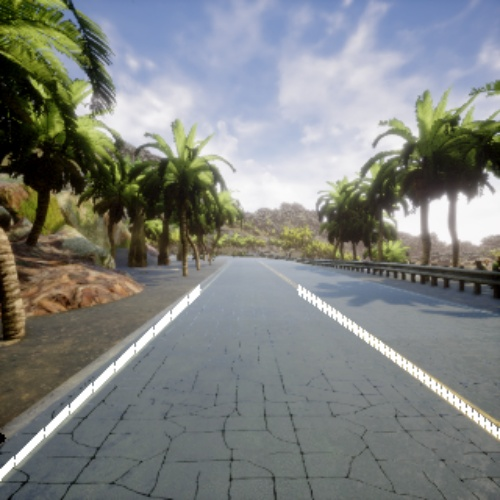
\includegraphics[scale=0.5]{figs/Diseño/Regresiones/Regresiones.jpg}
  \end{center}
  \caption{Resultado de la regresión cuadrática}
  \label{fig:regresión cuadrática}
\end{figure}\

\subsection{Interpolación y cálculo del centro de masas del carril}
\label{sec:Interpolación y cálculo del centro de masas del carril}

Para poder saber qué puntos se encuentran dentro de ambas regresiones cuadráticas, se realiza una interpolación. La interpolación consiste en recorrer
los puntos de la imagen original y quedarnos con los puntos que se encuentren dentro de los límites de ambas regresiones. Se realiza dos interpolaciones, una interpolación para 
los puntos de la regresión de la  derecha
y otra interpolación para los puntos de la regresión izquierda. Estas funciones interpolan los valores de los puntos en y en función de los valores de los puntos en x, más adelante se evalúa los valores de las puntos que se encuentran entre 
ambas regresiones cuadráticas como se muestra en el código \ref{cod:interpolación}. Cuando se proceda a dicha evaluación, se desarrolla un filtro para seleccionar el rango de puntos que representar un fragmento del carril de color azul en la imagen
final. Visualizando el resultado en la figura \ref{fig:interpolación} \newline

\begin{code}[h]
  \begin{lstlisting}[language=Python]

    def interpolate_lines(self,cvimage,points_line_left,points_line_right):


    gray_image = cv2.cvtColor(cvimage, cv2.COLOR_BGR2GRAY) 

    np_gray = np.array(gray_image)

    x, y = np.nonzero(np_gray)


    img_points = np.column_stack((x, y))

    f1 = interp1d(points_line_left[:, 0], points_line_left[:, 1],kind='slinear',fill_value="extrapolate")
    f2 = interp1d(points_line_right[:, 0], points_line_right[:, 1],kind='slinear',fill_value="extrapolate") 
    y_values_f1 = f1(img_points[:, 0])
    y_values_f2 = f2(img_points[:, 0])
    indices = np.where((y_values_f1 < img_points[:, 1]) & (img_points[:, 1] <= y_values_f2))
    
    
    points_between_lines = img_points[indices]
    filtered_points_between_lines = points_between_lines[points_between_lines[:,0] > 180]
    return filtered_points_between_lines
    

  \end{lstlisting}
  \caption[Método de interpolación]{Método del cálculo de las funciones de interpolación}
  \label{cod:interpolación}
  \end{code}  



  \begin{figure} [H]
    \begin{center}
      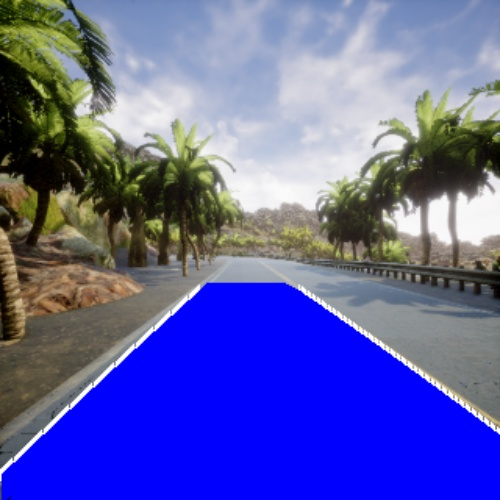
\includegraphics[scale= 0.5]{figs/Diseño/Regresiones/Interpolacion.jpg}
    \end{center}
    \caption{Resultado de la interpolación}
    \label{fig:interpolación}
  \end{figure}\

  Finalmente, cuando obtengamos el cálculo del carril que queremos seguir solamente faltará calcular el centro de masas de dicho fragmento conocido como el centroide siguiendo la ecuación
  del cálculo de centro de masas de una superficie: \newline
  

  \begin{equation} 
    \vec{r}_{CM} = \frac{\sum_{i}m_{i} \vec{r}_{i}}{\sum_{i}m_{i}} = \frac{\sum_{i}m_{i} \vec{r}_{i}}{M} 
    \newline
  \end{equation} 
  \newline
  Supondremos que todos los puntos tienen la misma masa (m\_i = 1). Esto simplifica el cálculo, pero en aplicaciones del mundo real, las masas pueden variar.
  El segundo paso es el cálculo de la masa total, se calcula multiplicando la masa individual (m\_i) por la cantidad de puntos en el carril. A continuación se calcula
  la suma de las posiciones de los puntos ponderadas por su masa y dividimos por la masa total calculada anteriormente. El resultado es una centro de masas conocido como centroide
  con coordenada x e y como se muestra en la figura final \ref{fig:centro de masas}. \newline

  \begin{figure} [H]
    \begin{center}
      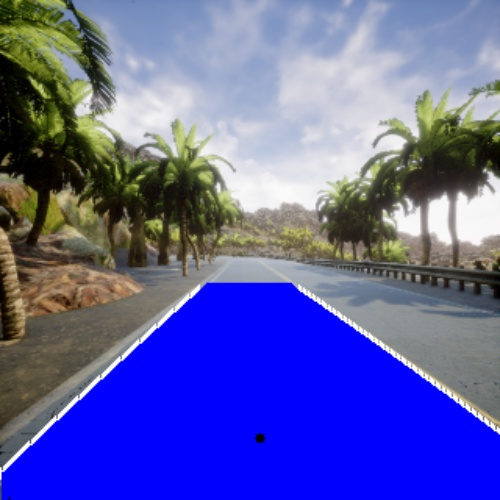
\includegraphics[scale=0.5]{figs/Diseño/Regresiones/centroide.jpg}
    \end{center}
    \caption{Resultado del centro de masas}
    \label{fig:centro de masas}
  \end{figure}\

  \subsection{Análisis del algoritmo de percepción}
  \label{sec:Análisis del algoritmo de percepción}
  Por último, realizamos un analisis de tiempos de cada parte para saber cuánto tiempo tarda en realizarse la percepción completa. Dicho análisis se llama profiling, con esta técnica 
  nos ayuda ver el rendimiento que podemos llegar a tener del algoritmo de percepción en cuanto a eficiencia. En la figura \ref{fig:centro de masas}, 
  se muestra una media de cuanto tarda cada componente de la percepción en segundos.


  \begin{figure} [H]
    \begin{center}
      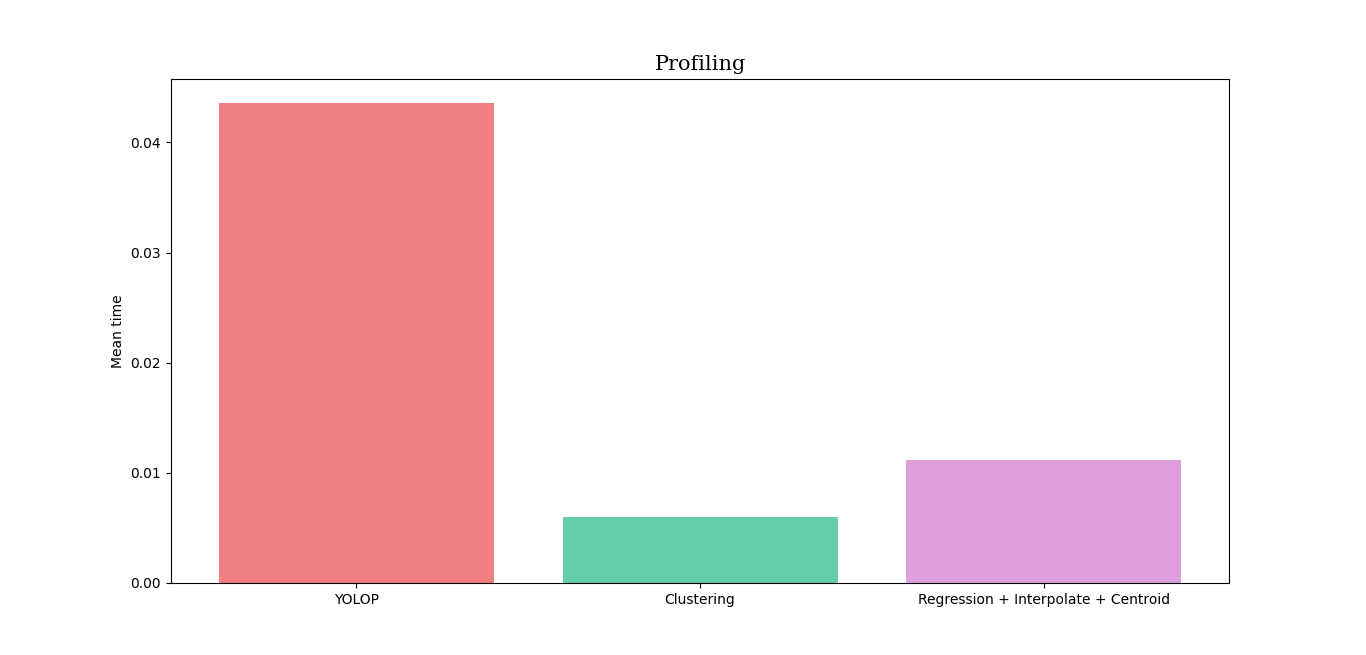
\includegraphics[scale=0.4]{figs/Diseño/Percepcion/time_profiling.png}
    \end{center}
    \caption{Profiling de las partes de la percepción}
    \label{fig:centro de masas}
  \end{figure}\

  Como podemos apreciar, la parte de la percepción que tarda más es el cálculo de la regresiones cuadráticas, la interpolación y el cálculo del centroide. Esto se debe a que
  cuando se realiza el cálculo de las regresiones hay que recorrer los puntos de los grupos de clústeres y cálcular sus funciones para obtener las regresiones. Respecto al 
  tiempo que tarda el algoritmo de DBSCAN junto con la clasficación de los clústeres es el ganador en cuanto menor tiempo de cómputo lo cual es interesante trabajar 
  con dicho algoritmo de clustering. En conclusión, sumando todos los tiempos de cada parte obtenemos un tiempo global de 0.033 segundos pasado a FPS conseguimos un rate aproximadamente
  de 30 FPS. 

  \section{Seguimiento del carril mediante control clásico}
  \label{sec:Control}

  Una vez realizado el comportamiento de la percepción, construiremos un comportamiento autónomo con el dron basandonos en un simple controlador PID. 
 Con este primer comportamiento queremos demostrar la funcionalidad de la percepción utilizando un controlador de movimiento sencillo. \newline

 Un controlador PID (proporcional, derivativo e integral) es un 
  es un sistema que es capaz de mantener una variable (como la temperatura, velocidad o posición) cercana a un valor deseado o de referencia. Cada componente de un controlador tiene un papel 
  importante,
  la componente P (proporcional) ajusta la salida del controlador en función de la diferencia entre el valor medido y el valor deseado. 
  Cuanto mayor sea esta diferencia (error), mayor será la corrección aplicada. Sin embargo, el control proporcional solo no puede eliminar completamente el error por ello se utiliza
  las componentes derivativa e integral. La componente D (derivativa) considera la tasa de cambio del error,
  si el error cambia rápidamente, el término derivativo aplicará una corrección para evitar oscilaciones o inestabilidad.
  Con el término integral se acumula el error a lo largo del tiempo y ajusta la salida del controlador en función de esta acumulación. 
  Ayuda a eliminar el error persistente o constante. Si el error es pequeño pero persistente, el término integral lo corregirá gradualmente.
  \newline

  Lo cual con este controlador PID sencillo se controlan las velocidades respecto al error que se produce entre posición deseada y la que obtenemos. La variable deseada para estar alineados con el carril se escoge
  el eje de las x el valor central de la imagen, ya que queremos en todo momento permanecer centrales respecto al carril. Para calcular el error se calcula la diferencia del valor deseado que seria 
  el valor central de la imagen y el valor del centroide del carril mencionado en la sección \ref{sec:Interpolación y cálculo del centro de masas del carril}. 
  A parte de este controlador, se utiliza un pequeño controlador PD para controlar la altura del vehículo y tengamos una altura medianamente constante. Para saber a qué altitud nos encontramos se utiliza el sensor del Lidar.

  Para encontrar los valores de cada término que compone ambos controladores se ha realizado a base de experimentación, empezando de manera creciente, es decir, primero utilizariamos
  la componente proporcional para ver su comportamiento, una vez que tengamos el valor del término proporcional pasaremos al término derivativo para suavizar los movimientos que puede
  producir este término y por último utilizariamos la parte integral para eliminar el error. El controlador PID se usará para controlar la velocidad de giro del dron en cuanto a la velocidad lineal 
  tendremos un valor constante. En el código \ref{cod:ValoresPID} se expone los valores de cada componente en ambos controladores.\newline

  \begin{code}[h]
    \begin{lstlisting}[language=Python]

      kp_height = 0.1
      kd_height = 0.4

      kp_speed_controller = 0.09
      kd_speed_controller = 0.1
      ki_speed_controller = 0.008
     
    \end{lstlisting}
    \caption[Valores de las variables del PD del control de altura y del PID del controlador de velocidad angular]{Valores de las variables del PD del control de altura y del PID del controlador de velocidad angular}
    \label{cod:ValoresPID}
    \end{code} 

  \section{Seguimiento del carril mediante aprendizaje por refuerzo}
  \label{sec:aprendizaje por refuerzo}

  Como mencionamos en la sección \ref{sec:IA},el aprendizaje por refuerzo consiste en enseñar un agente 
  desempeñar un comportamiento mediante recompensas y penalizaciones. Este comportamiento se aprende a base de interacciones con el entorno de trabajo y observaciones de como puede responder,
  de forma similar a los niños que exploran el mundo que les rodea y aprenden las acciones que les ayudan a alcanzar un objetivo. Se compone de diferentes elementos claves que se definen
  al problema a resolver del seguimiento del carril:
  \begin{itemize} 
    \item \textbf{Agente}: El agente es una entidad o modelo que pretendemos entrenar para que aprenda a tomar decisiones (acciones) en función del estado en el que nos encontremos. Nuestro 
    agente se trata del dron.
    \item \textbf{Entorno}: Ambiente en donde interactua el agente para que pueda aprendar el comportamiento deseado. El dron estará interectuando sobre el entorno de Coastline que nos proporciona Airsim 
    durante las fases de pruebas. 
    \begin{figure} [H]
      \begin{center}
        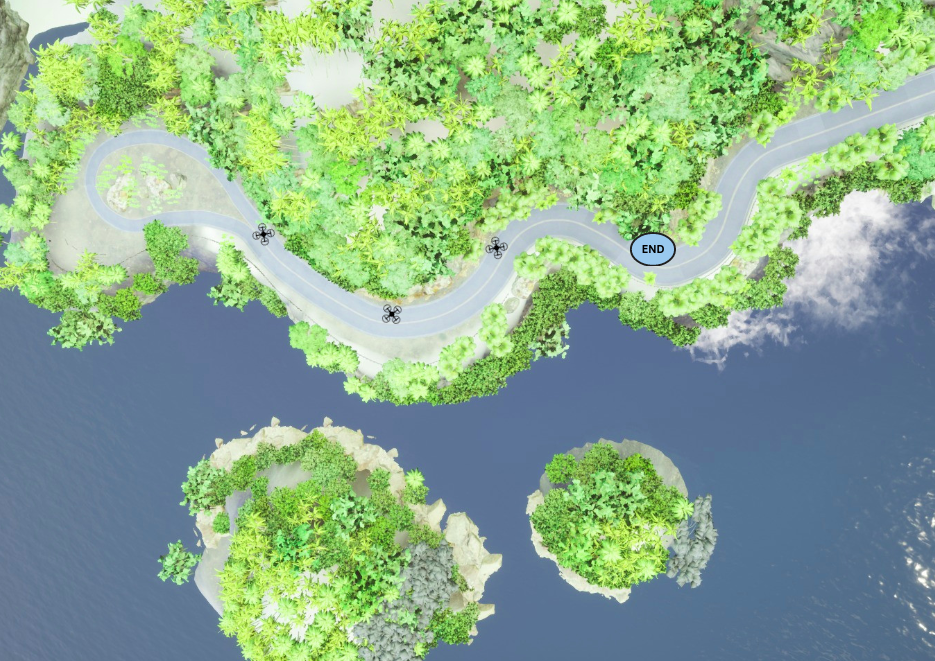
\includegraphics[scale=0.4]{figs/Diseño/RL/entorno.png}
      \end{center}
      \caption{Entorno en la fase de entrenamiento del sigue carril basado en Q-Leaning}
      \label{fig:Entorno}
    \end{figure}\

    Dentro de este circuito, hemos escogido tres localizaciones distintas para el vehículo a la hora de realizar el entrenamiento con el algoritmo de Q-Learning y el punto final del recorrido. Como se puede apreciar en la figura \ref{fig:Entorno} las posiciones
    tienen una distancia entre ellas considerablemente. 
    \item \textbf{Estados}: Condiciones en las que se puede encontrar el agente en ese instante de tiempo. Para la definición de los estados, se divide la imagen que damos como la salida de la detección del carril en 14 franjas, dichas franjas tienen una 
    separación de 10 pixeles. Las franjas representan cada estado en el que se puede encontrar el agente. Empezamos a definir el primer estado desde la izquierda hasta la derecha con una
    hasta conseguir los 14 estados correspondientes, 7 estados izquierda, 1 estado central y 6 estados derecha. Se puede observar el resultado de los estados en la figura \ref{fig:Estados}

    \begin{figure} [H]
      \begin{center}
        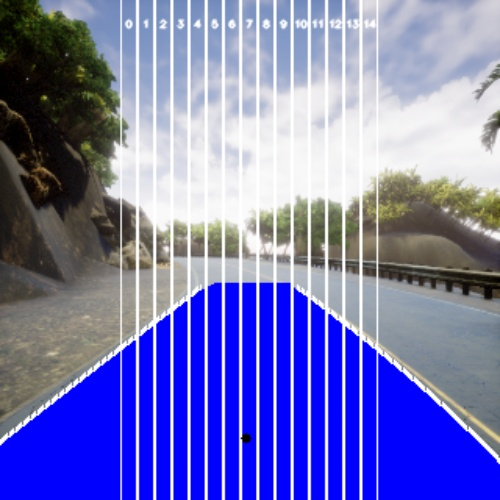
\includegraphics[scale=0.5]{figs/Diseño/RL/estados.jpg}
      \end{center}
      \caption{Estados definidos para el sigue carril basado en Q-Learning}
      \label{fig:Estados}
    \end{figure}\

    \item \textbf{Acciones}: Movimientos que puede realizar el agente dentro del estado en el entorno de entrenamiento. En total, se definen 21 acciones, que podrá escoger el agente en el algoritmo de Q-Learning. Se componen de pares de velocidades lineales y angulares, las velocidades lineales
    tendrán un intervalo de 0.1 m/s hasta 2.0 m/s. Así siendo el intervalo de la velocidad angular de -25 hasta 25 grados/segundo, teniendo giros hacia la izquierda y hacia la derecha. Dichos pares
    de velocidades serán formados a partir de la función que nos proporciona numpy llamada linspace\footnote{\url{https://numpy.org/doc/stable/reference/generated/numpy.linspace.html}}. \newline
  
    \begin{code}[H]
      \begin{lstlisting}[language=Python]
  
        
        def build_actions():
            ACTIONS = []
            speeds_actions = np.linspace(0.1,2.0,11, dtype=float)
            angular_speeds = np.linspace(-25,25, 21)
        
            left_angular_speeds = angular_speeds[:10]
            right_angular_speeds = np.flip(angular_speeds[-10:])
            central_angular_speed = angular_speeds[10]
            speeds = speeds_actions[:10]
            central_speed = speeds_actions[10]
        
            for i in range(len(speeds)):
                ACTIONS.append([round(speeds[i],3),round(left_angular_speeds[i],3)])
        
            ACTIONS.append([round(central_speed,3),0.0])
        
            for  i in reversed (range(len(speeds))):
                ACTIONS.append([round(speeds[i],3),round(right_angular_speeds[i],3)])
  
            return ACTIONS
       
      \end{lstlisting}
      \caption[Construcción de las acciones para Q-Learning]{Construcción de las acciones para Q-Learning}
      \label{cod:Acciones}
      \end{code}
      
    \item \textbf{Función de Recompensa o Penalizaciones}: Consiste en como queremos premiar o penalizar al agente con el objetivo que queremos cumplir. Las recompensas o penalizaciones se recogen
    en una función, dicha función es independiente en cada diseño del objetivo que quiere completar el agente. La función de recompensa se compone de dos partes premiando al dron de que
    permanezca centrado en el carril y además preamiarle por mantener una orientación adecuada respecto al carril, asegurando que se navegue de forma paralela al mismo. Cada parte tiene un peso
    de importancia, siendo el peso que se permanezca del carril del 85\% y la orientación respecto al carril de un 15\%. Tanto la recompensa por mantenerse centrado en el carril 
    como la orientación respecto al carril es normalizada entre valores de 0-1, penalizando con un valor constante al dron cuando se salga del carril o 
    se pierda la percepción. La implementación de la función de recompensa y las penalizaciones se puede ver en el código \ref{cod:recompensa}:

    \begin{code}[H]
      \begin{lstlisting}[language=Python]
  
        def reward_function(self,cx,angle):

        reward = 0
        target_heading = 0
        error_lane_center = (WIDTH/2 - cx)
        heading_difference = (target_heading - angle) 
        
        MIN_ERROR = 0
        MAX_ERROR = 80

        MIN_ANGLE = 0
        MAX_ANGLE = 70

        CENTRE_WEIGHT = 0.85
        ANGLE_WEIGHT = 0.15
        
        if (self.is_exit_lane(cx)):
            
            reward = -10

        else:

            
            normalise_error_centre = (abs(error_lane_center) - MIN_ERROR) / (MAX_ERROR - MIN_ERROR)
            reward_centre = 1 - normalise_error_centre

            
            normalise_error_angle = (abs(heading_difference) - MIN_ANGLE) / (MAX_ANGLE - MIN_ANGLE)
            reward_angle = 1 - normalise_error_angle


            reward = (reward_centre * CENTRE_WEIGHT) + (reward_angle * ANGLE_WEIGHT)
            
        return reward
       
      \end{lstlisting}
      \caption[Función de recompensa]{Función de recompensa}
      \label{cod:recompensa}
      \end{code}
    \item \textbf{Política}: Determina que acción realizar en cada estado que se encuentre el agente. Dicha política varía según el tipo de algoritmo que queremos seguir dentro de aprendizaje por refuerzo.
    Puede ser determinista o estocástica.

    En este TFG, se sigue una política epsilon-greedy\cite{Epsilon-greedy}, que consiste 
 equilibrar la exploración y explotación en la fase de entrenamiento. Cuando el agente tenga que escoger la acción que tomar tendra en cuenta dos enfoques:
 
 \begin{itemize}
   \item Exploración (con probabilidad $\epsilon$): El agente escogerá una acción al azar para explorar
   \item Explotación(con probabilidad $ 1 - \epsilon$): El agente escogerá la acción con el valor de la tabla Q(S,A) más alto, es decir, la mejor acción conocida
 \end{itemize}
 
 El parámetro $\epsilon$ es el responsable de controlar la proporción de exploración frente a explotación, si $\epsilon$ es alto el agente explorará más en cambio si $\epsilon$ es bajo
 el agente se centrará en la explotación. Por lo que en la elección de acción se generará un numero n aleatoriamente, si n es menor que la probabilidad $\epsilon$ la acción se escogerá aleatoriamente
 en cambio si n es mayor que la probabilidad de $\epsilon$ la acción será que mayor valor tenga en la tabla Q(S,A) para dicho estado. \newline
 
 Dentro de esta política la probabilidad de $\epsilon$ será decayente, es decir, no tener un valor constante en cada episodio que nos encontremos, lo que realizaremos es una disminuición 
 de esta probabilidad para conseguir que el agente con el paso del tiempo poco a poco explote lo que ha aprendido y que el modelo llegue a una convergencia óptima. Para llevar a cabo el descenso
 de $\epsilon$ se puede realizar de varias formas, por ejemplo podemos realizarlo linealmente, logaritmicamente, exponencial o escalonado. \newline
  \end{itemize}

  El algoritmo Q-Learning se basa en seguir una función acción-recompensa formada por un tabla estado-acción la cual iremos rellenando siguiendo la siguiente ecuación
  de Bellman\cite{Bellman}:
  
  \begin{equation}
    Q(s, a) = Q(s, a) + \alpha \cdot [R(s, a) + \gamma \cdot \max Q(s', a') - Q(s, a)]
  \end{equation}

  en donde, 

  \begin{itemize}
    \item \textbf{$Q(s, a)$}: Valor Q para el estado $s$ y la acción $a$. Se trata de una matriz formada por estado y acción.
    \item \textbf{$\alpha$}: Tasa de aprendizaje entre un valor de 0 a 1. Consiste en el porcentaje que daremos al agente para el proceso de aprendizaje, 
    si dicho valor es alto daremos más peso al valor aprendido. Dicho valor se define con un valor de 0.5 
    \item \textbf{$R(s, a)$}: Recompensa por tomar la acción $a$ en el estado $s$. La función de recompensa es crucial en el proceso de aprendizaje del agente, evalua como es favorable o deseable
    es una acción tomada por el agente en el estado que se encuentre. Proporciona información al agente sobre que acciones maximizan la recompensa total a lo largo del tiempo. Dicha función
    de recompensa es diseñada dependiendo de cual sea el objetivo de tu agente. 
    \item \textbf{$\gamma$}: Factor de descuento entre un valor de 0 a 1. Modela la importancia de las recompensas futuras en relación con las recompensas inmediatas, refleja la importancia del agente
    por las recompensas a largo plazo. Un valor alto sifnigicará que le agente valorará mucho las recompensas futuras, mientras que un valor bajo indica que se enfocará más en las recompensas
    inmediatas. Dicho valor se define con un valor de 0.7.
    \item \textbf{$\max Q(s', a')$}: Valor Q máximo en el próximo estado $s'$ para todas las acciones posibles $a'$.
\end{itemize}

A la medida que vayamos avanzando en la fase de entrenamiento, iremos rellenando la tabla Q(s,a) para más adelante indexar en ella en la fase de inferencia.

\subsubsection{Fase de entrenamiento}
\label{sec:fases_ql}
 Antes de adentrarnos en esta fase, definiremos dos conceptos importantes:
 \begin{itemize}
  \item \textbf{Episodios}: Se define episodio como una secuencia completa de interacciones que se produce entre el agente y el entorno. Cada episodio comienza con un estado inicial y consta de una serie 
  de pasos o acciones tomadas por el agente.
  \item \textbf{Iteraciones (steps)}: Son los pasos que puede dar un agente en el entorno dentro de un episodio. Estos pasos pueden incluir observaciones del entorno, decisiones tomadas por el agente
  y las consecuentes recompensas o penalizaciones recibidas.
\end{itemize}

 
 La fase de entrenamiento consiste en el que el agente explore todo lo máximo posible en el entorno respecto a los estados que tiene y las acciones que puede tomar, es decir, al comienzo del entrenamiento se inicializará la tabla Q(S,A) a cero todos sus valores, esta representación
 al comienzo es así ya que el agente desconoce por completo el entorno hasta que poco a poco vaya iterando sobre él en cada estado tomando x accion. \newline
 
 Basicamente, en cada iteración del algoritmo se escogerá una acción según si estamos en exploración o explotación, se calculará la recompensa obtenida e iteraremos de nuevo sobre el algoritmo.

 El entrenamiento finaliza cuando el agente haya aprendido el objetivo que queremos seguir, esto se sabe cuando las iteraciones del algoritmo y la recompensa acumulada del agente en esta 
 fase se estabilice y tenga valores constantes, es decir, no cambia significativamente con más iteraciones, esto se denomina que el modelo ha convergido y pasaremos a la fase de inferencia. \newline

Durante esta fase, dejamos el algoritmo de Q-Learning entrenando durante aproximadamente 12 horas teniendo un rate del algoritmo de Q-Learning más el algoritmo de percepción aproximadamente de 
unos 10 FPS. De esta manera, nos podemos asegurar que el algoritmo completará el entrenamiento de manera correcta y poco a poco 
acabará convergiendo. 
En la figura \ref{fig:entrenamiento} se ilustra la fase de entrenamiento durante la navegación del dron. En la primera figura se corresponde al número de iteraciones de cada 
episodio durante el entrenamiento, la segunda corresponde al valor que va teniendo épsilon en cada episodio y la tercera grafica se muestra el valor de la recompensa 
acumulativa en cada episodio. \newline

\begin{figure} [H]
  \begin{center}
    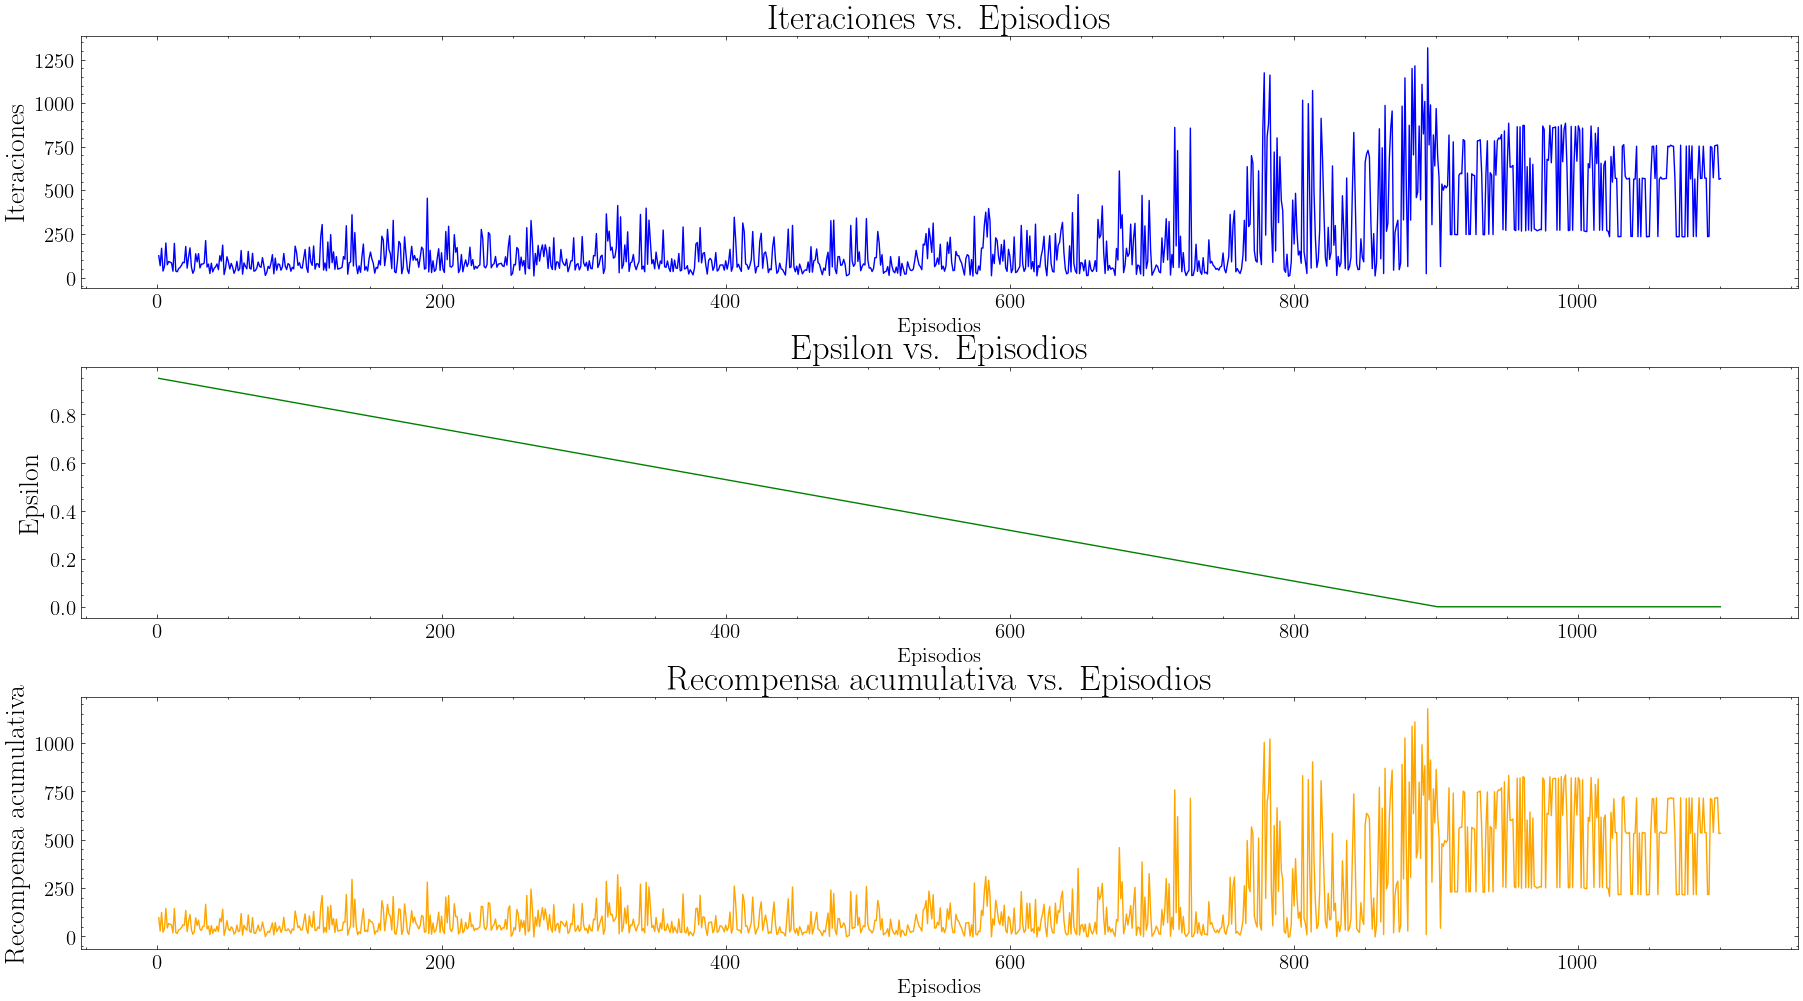
\includegraphics[scale=0.35]{figs/Diseño/RL/graficas-entrenamiento.png}
  \end{center}
  \caption{Gráficas de la fase de entrenamiento}
  \label{fig:entrenamiento}
\end{figure}\

Al comienzo del entrenamiento, se puede observar que el dron obtiene pocas iteraciones y bajas recompensas acumulativas, 
esto se debe a que el dron al comienzo del entrenamiento desconoce por completo el entorno. A medida que vamos avanzando en el entrenamiento, 
las iteraciones y los valores de la recompensa acumulativa son mayores hasta que en el episodio 900 donde acaba la fase de exploración 
siendo el valor de épsilon cero (las acciones no son aleatorias). A partir de ese punto, la recompensa y las iteraciones tienen una tendencia ascendente, y finalmente, 
a lo largo del entrenamiento, ambas se estabilizan en un valor fijo sin cambiar considerablemente. Esto se debe a que el dron completa constantemente el circuito en cualquier
punto de reinicio dentro del circuito mostrado en la figura \ref{fig:Entorno} sin cambiar considerablemente la tabla Q. En este momento, se puede decir que el algoritmo ha sido capaz de converger. Una vez se analice 
los resultados del entrenamiento con las diferentes métricas daremos pie a la fase de inferencia para verificar el resultado obtenido con el modelo entrenado. 

\subsubsection{Fase de inferencia}
\label{sec:fases_inferencia}
La fase de inferencia consiste en indexar la tabla Q(S,A) que hemos ido rellenando en la fase de entrenamiento. El dron cuando se encuentré en un estado especifico consultará la tabla Q(S,A) para
encontrar la mejor acción en ese estado (cuando mencionamos la mejor acción nos referimos al máximo valor en la tabla que tenga en ese estado). Cuando el dron tome dicha acción se moverá al siguiente estado
siendo así un proceso iterativo hasta alcanzar la meta. En esta fase, los valores de la tabla permanecen constantes y se utiliza para la toma de decisiones basadas en el conocimiento
aprendido en la fase de entrenamiento. \newline

En la figura \ref{fig:Distribucción_inferencia} se puede observar las diferentes acciones que ha utilizado el dron para completar el circuito de entrenamiento utilizando cuatro de veintiuno de acciones
disponibles. Se destaca que la acción más usada se trata de una de las acciones que presentan poco giro y alta velocidad lineal dentro de las acciones con más velocidad lineal, esto se debe
a la importancia de la función de recompensa al considerar que queremos que el dron se mantenga constantemente en el centro del carril manteniendo un angulo de orientación adecuado
sin salirse del carril.

\begin{figure} [H]
  \begin{center}
    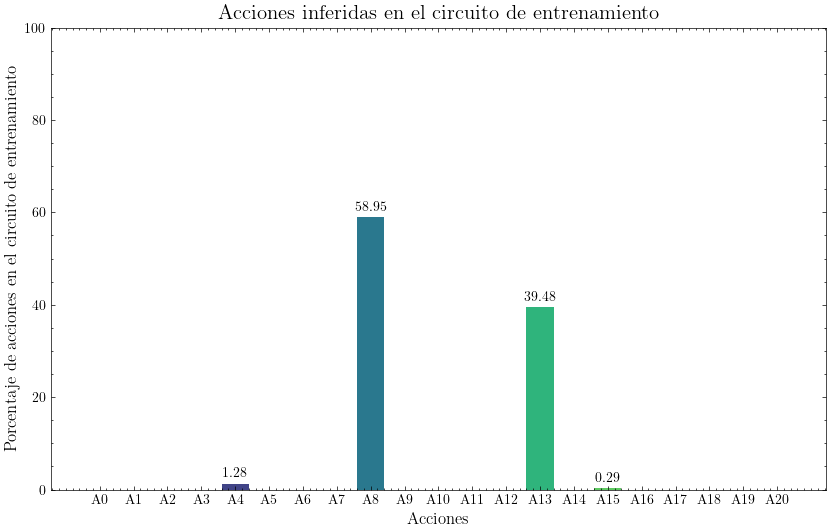
\includegraphics[scale=0.7]{figs/Diseño/RL/Acciones_inferidas.png}
  \end{center}
  \caption{Distribucción de acciones en el circuito de entrenamiento}
  \label{fig:Distribucción_inferencia}
\end{figure}\

Como resultado al utilizar el algoritmo de Q-learning, el modelo entrenado ofreció ser un resultado eficaz a la hora de navegar por el circuito, pudiendo observar 
el modelo entrenado final en diferentes localizaciones alteatorias en el entorno de la figura \ref{fig:Entorno}. Para poder obtener el máximo rendimiento del modelo entrenado se busco los límites de velocidad
angular y lineal a la que podía ir el dron, esto significa multiplicar por un factor todas las acciones tanto las velocidades lineales y angulares. Este proceso es interesante 
realizarlo para maximizar el comportamiento sin la necesidad de volver a entrenar un nuevo modelo. Estos factores se pueden ver en el código \ref{cod:Factores} lo cual 
las acciones se pueden aumentar un 100\% lo que podemos decir que el modelo entrenado es efectivo al aumentar el valor de las acciones. \newline

\begin{code}[h]
  \begin{lstlisting}[language=Python]

    factor_speed = 2.0
    factor_angular_speed = 1.8
   
  \end{lstlisting}
  \caption[Factores]{Valores de los factores aplicados a las acciones de Q-learning}
  \label{cod:Factores}
  \end{code} 

Siendo los nuevos valores de las acciones utilizados durante las fases de comparación entre el seguimiento de carril con el PID y el seguimiento de carril mediante Q-Learning. Los nuevos
valores de las acciones originales como se mostraba en el código \ref{cod:Acciones} son multiplicados por ambos factores
y su gráfico de acciones como se muestra en la figura \ref{fig:inferencia_factor}. Se puede observar que en la distribución de acciones el dron
sigue escogiendo acciones con velocidad lineal alta y velocidad angular baja para mantenerse dentro del recorrido sin salirse, además de aumentar el porcentaje de las acciones escogidas respecto a la distribución de acciones
que se mostraba en la figura \ref{fig:Distribucción_inferencia}

\begin{figure} [H]
  \begin{center}
    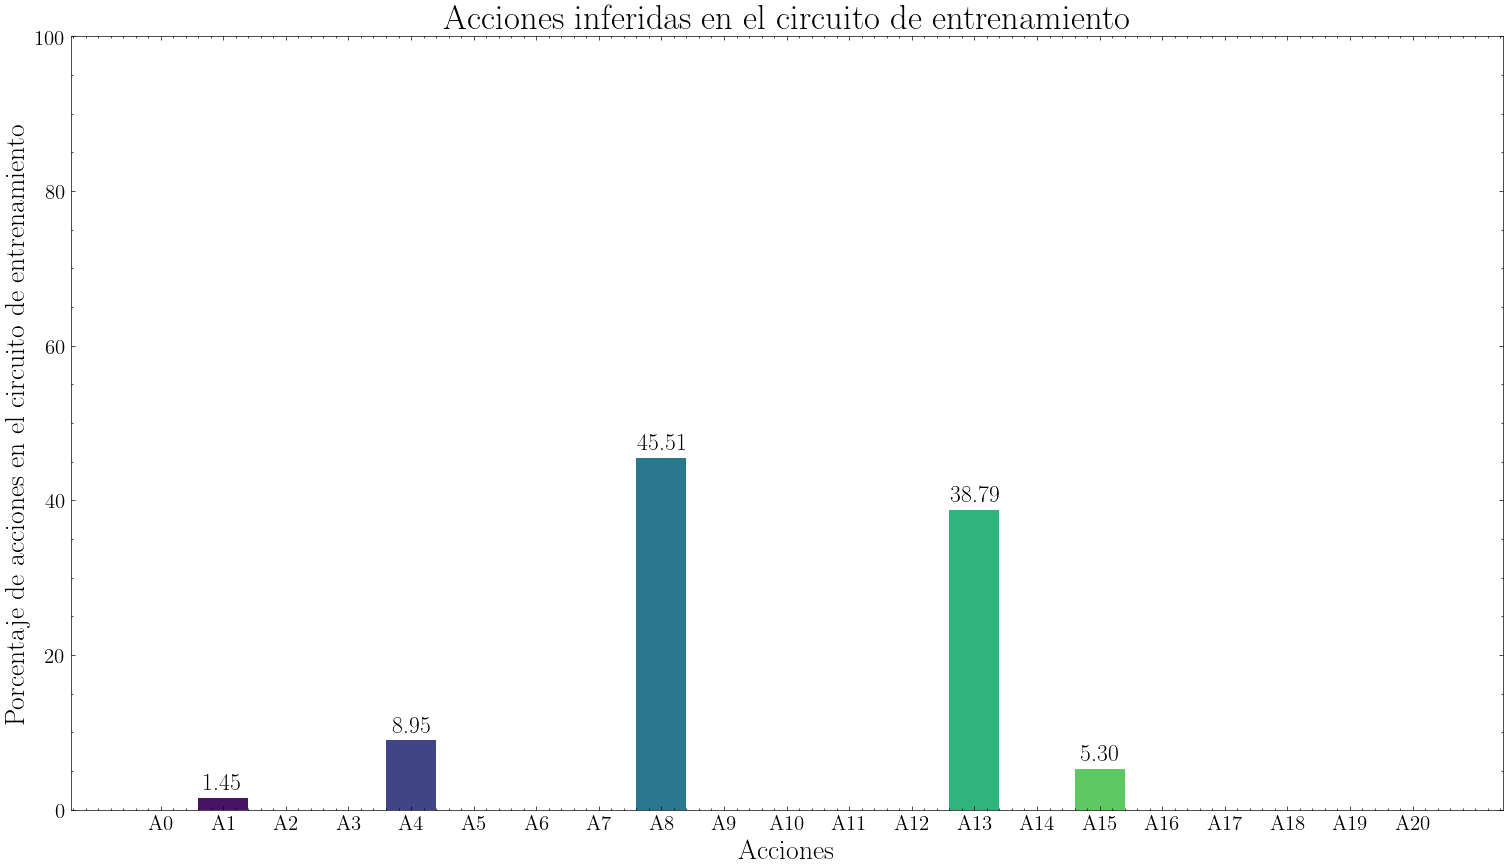
\includegraphics[scale=0.4]{figs/Diseño/RL/Acciones_inferidas_factor.png}
  \end{center}
  \caption{Distribucción de acciones en el circuito de entrenamiento multiplicadas por el factor}
  \label{fig:inferencia_factor}
\end{figure}\


\subsection{Análisis y comparativa entre el seguiento de carril clásico}
\label{sec:Análisis y comparativa entre el seguiento de carril clásico}
Para comprobar la robustez y la eficacia que demuestra ser el modelo entrenado junto con el seguimiento de carril mediante el PID, se realizo varias comparativas en ambos
comportamientos. Se ajusto las velocidades del controlador PID para que ambos tuviesen las mismas condiciones, para ello se utilizo un circuito en el que ambos son capaces 
de recorrerlo sin salirse del carril. En la figura \ref{fig:comparativa} se muestra el resultado de ambos comportamientos, en la primera figura es todo el recorrido hasta el punto
final y en la segunda figura se realiza zoom en una parte del recorrido, los datos fueron recogidos mediante la posición del dron guardandolos un fichero tanto las coordenadas 
en el eje x como las coordenadas en el eje y. 
  
\begin{figure}[H]
  \centering
  \begin{minipage}{1.0\textwidth}
    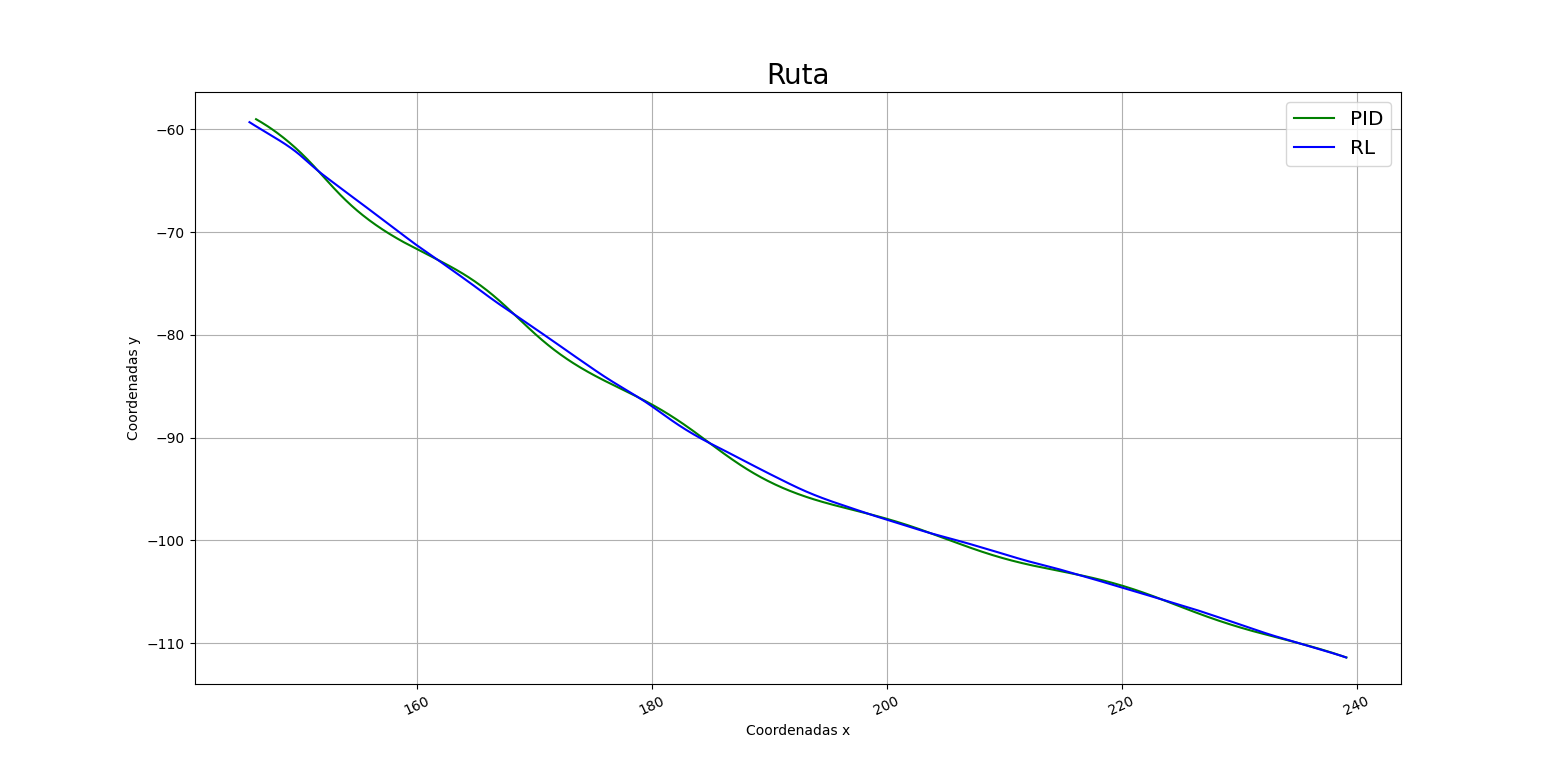
\includegraphics[width=\linewidth]{figs/Diseño/RL/ruta.png}
  \end{minipage}
  \hfill
  \begin{minipage}{1.0\textwidth}
    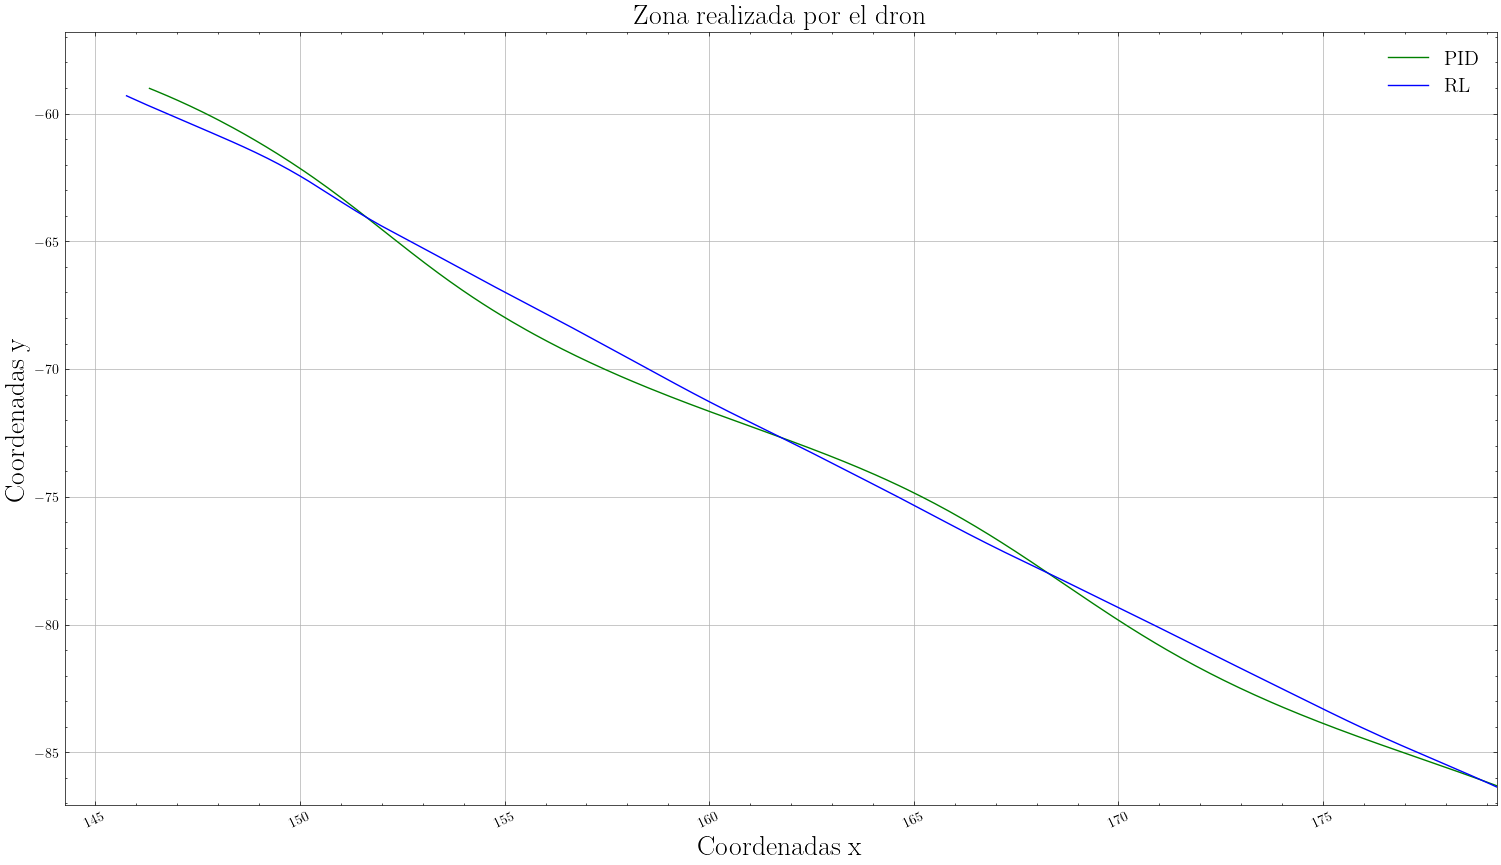
\includegraphics[width=\linewidth]{figs/Diseño/RL/ruta_zoom.png}
  \end{minipage}
  \caption{Comparativa realizando un trayecto entre ambos comportamientos}
  \label{fig:comparativa}
\end{figure}

Una de las principales diferencias entre ambos comportamientos es que el comportamiento con control clásico presenta oscilaciones durante el recorrido relizando eses 
por ambas partes del recorrido hasta llegar al punto final del recorrido. En cambio, el comportamiento con aprendizaje por refuerzo destaca por su trayectoria constante 
durante todo el recorrido sin apenas realizar oscilaciones, destacando que el trayecto para realizar la comparativa se trata de un trayecto recto sin apenas curvas que se 
puede visualizar en la figura \ref{fig:trayectoPID}.

\begin{figure} [H]
  \begin{center}
    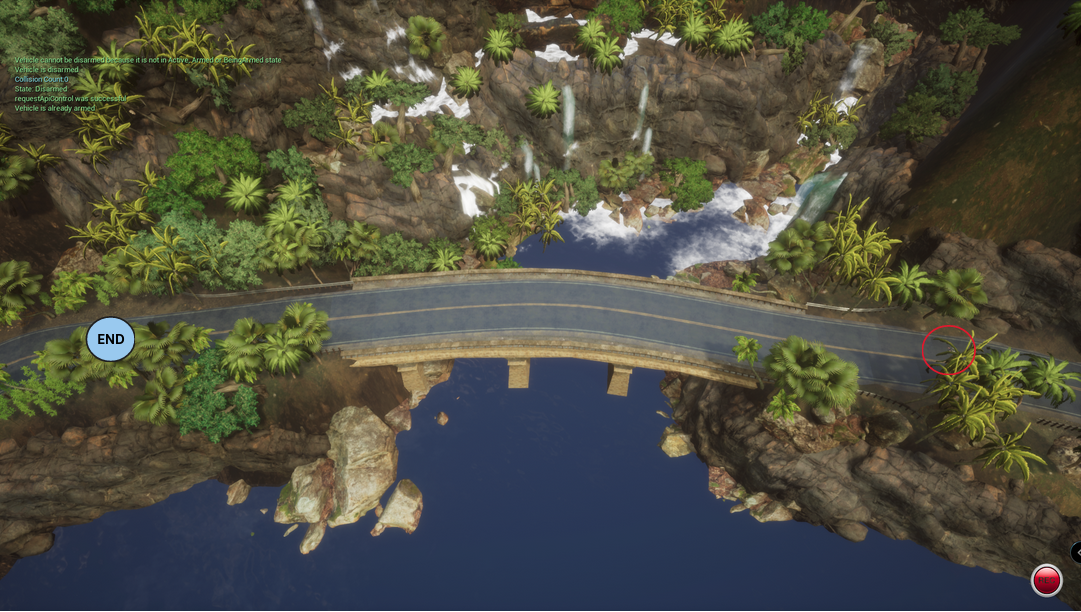
\includegraphics[scale=0.4]{figs/Diseño/RL/trayecto1.png}
  \end{center}
  \caption{Trayecto en donde se realiza la comparativa entre el PID y aprendizaje por refuerzo}
  \label{fig:trayectoPID}
\end{figure}\

Finalmente, en la figura \ref{fig:media_velocidades} se ilustra la media de velocidades angulares que han obtenido ambos comportamientos en el recorrido. Dichas velocidades
se han ido almacenando a la medida que el dron recorría el trayecto. Se puede apreciar como el comportamiento de aprendizaje por refuerzo obtiene menor media de velocidad angular respecto al controlador PID manteniendo un trayectoria segura y eficaz en un recorrido 
que nunca ha visto durante la fase de entrenamiento sin realizar apenas oscilaciones durante todo el trayecto. Respecto, al controlador PID, mantiene una media angular alta debido a que 
necesita realizar ajustes para mantenerse en el trayecto constantemente resultando tener una mayor giro para permanecer central al carril. \newline
En este tipo de trayectos, el comportamiento de aprendizaje por refuerzo demuestra ser más eficiente que el controlador PID sin requerir muchos ajustes respecto a la velocidad
angular para manterse en la trayectoria y es capaz de adaptarse a cualquier recorrido del entorno.

\begin{figure} [H]
  \begin{center}
    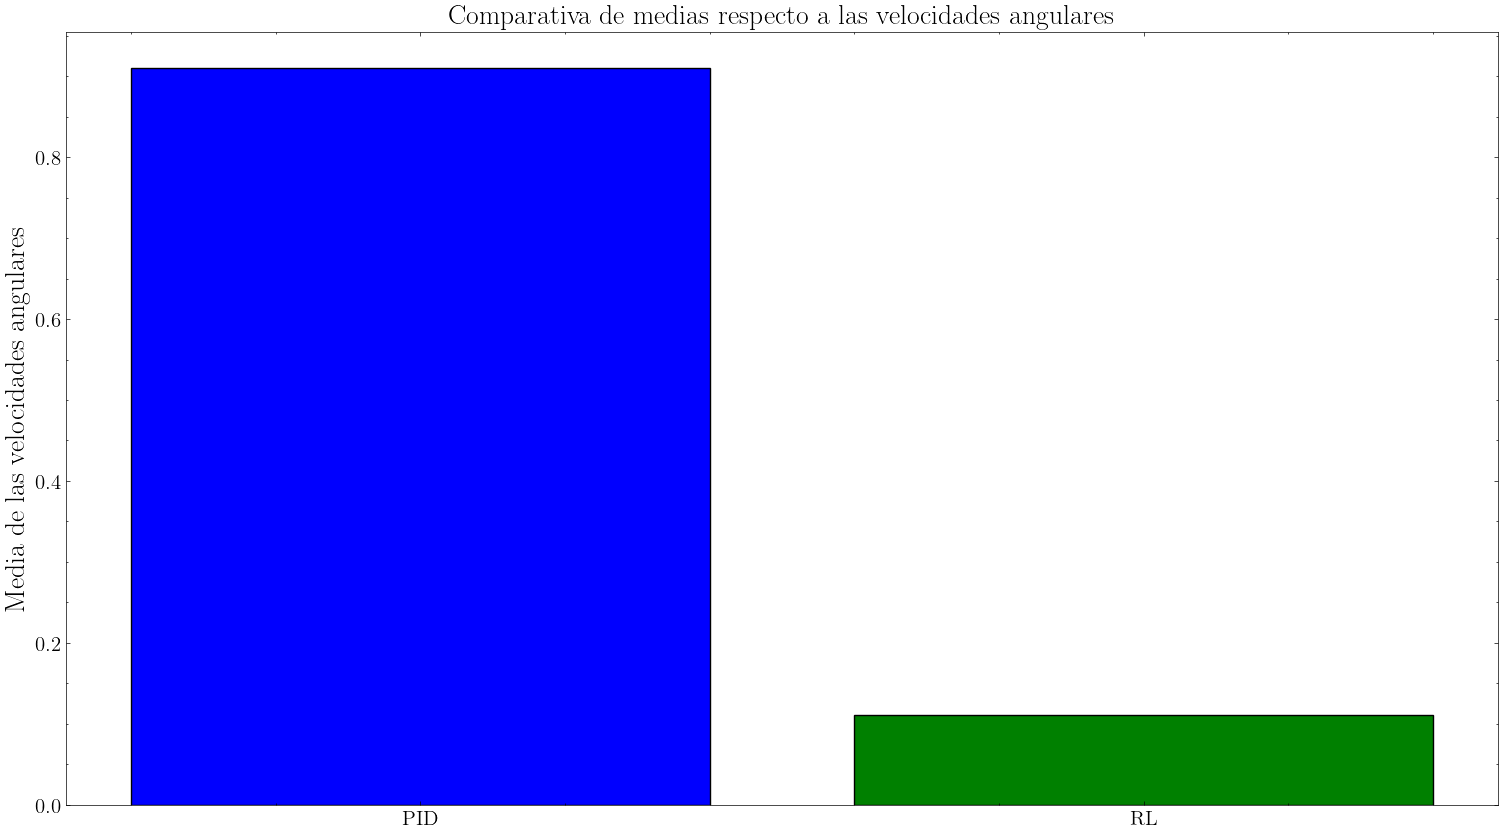
\includegraphics[scale=0.4]{figs/Diseño/RL/medias_velocidades_angulares.png}
  \end{center}
  \caption{Media de velocidades angulares de ambos comportamientos desarrollados}
  \label{fig:media_velocidades}
\end{figure}\

Demostrando asi que el modelo entrenado es capaz de obtener comportamientos satisfactorios tomando acciones acordes
al recorrido de entrenamento u recorridos que no ha visto durante en la fase de entrenamiento. En la figura \ref{fig:comparativa}, se muestra diferentes frames 
durante el recorrido siendo capaz de manternerse centrado al carril. 

\begin{figure}[H]
  \centering
  \begin{minipage}{0.3\textwidth}
    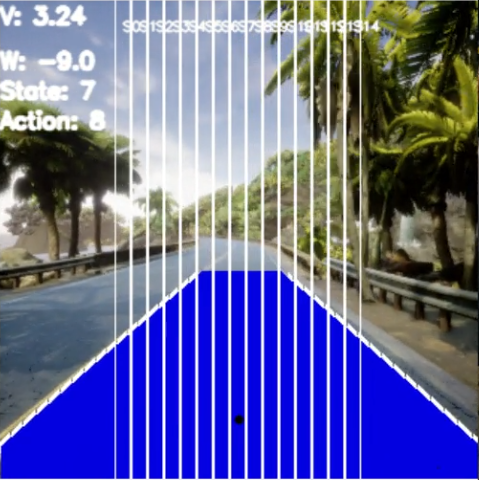
\includegraphics[width=\linewidth]{figs/Diseño/RL/rl1.png}
  \end{minipage}
  \hfill
  \begin{minipage}{0.3\textwidth}
    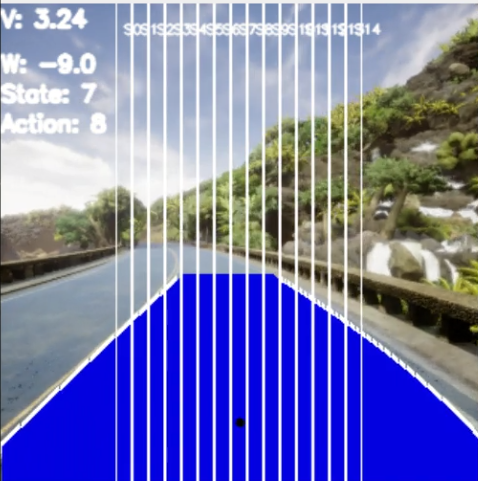
\includegraphics[width=\linewidth]{figs/Diseño/RL/rl2.png}
  \end{minipage}
  \hfill
  \begin{minipage}{0.3\textwidth}
    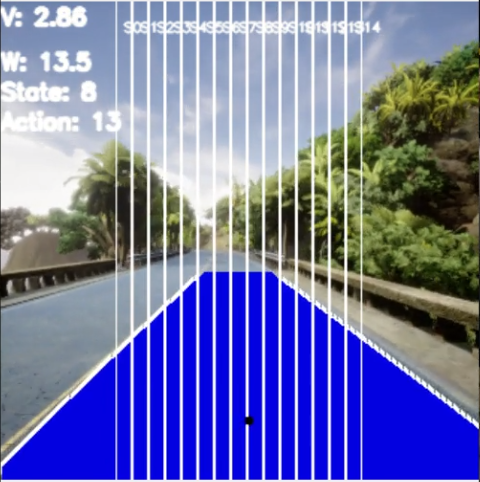
\includegraphics[width=\linewidth]{figs/Diseño/RL/rl3.png}
  \end{minipage}
  \caption{Resultado del comportamiento de aprendizaje por refuerzo ilustrando los estados y acciones teniendo en cuenta el factor}
  \label{fig:comparativa}
\end{figure}














        


  

